\documentclass{article} 
\usepackage{polski} %moze wymagac dokonfigurowania latexa, ale jest lepszy niż standardowy babel'owy [polish] 
\usepackage[utf8]{inputenc} 
\usepackage[OT4]{fontenc} 
\usepackage{graphicx,color} %include pdf's (and png's for raster graphics... avoid raster graphics!)
\usepackage{url}
\usepackage{listings}
\usepackage{enumerate}
\usepackage[pdftex,hyperfootnotes=false,pdfborder={0 0 0}]{hyperref} %za wszystkimi pakietami; pdfborder nie wszedzie tak samo zaimplementowane bo specyfikacja nieprecyzyjna; pod miktex'em po prostu nie widac wtedy ramek

% Zmiana rozmiarów strony tekstu
\addtolength{\voffset}{-1cm}
\addtolength{\hoffset}{-1cm}
\addtolength{\textwidth}{2cm}
\addtolength{\textheight}{2cm}

%bardziej zyciowe parametry sterujace rozmieszczeniem rysunkow
\renewcommand{\topfraction}{.85}
\renewcommand{\bottomfraction}{.7}
\renewcommand{\textfraction}{.15}
\renewcommand{\floatpagefraction}{.66}
\renewcommand{\dbltopfraction}{.66}
\renewcommand{\dblfloatpagefraction}{.66}
\setcounter{topnumber}{9}
\setcounter{bottomnumber}{9}
\setcounter{totalnumber}{20}
\setcounter{dbltopnumber}{9}

% własny bullet list z malymi odstepami
\newenvironment{tightlist}{
\begin{itemize}
  \setlength{\itemsep}{1pt}
  \setlength{\parskip}{0pt}
  \setlength{\parsep}{0pt}}
{\end{itemize}}

%obrazkow szukamy w nastepujacym katalogu:
\graphicspath{{pics/}}



\begin{document}

\thispagestyle{empty} %bez numeru strony

\begin{center}
{\large{Sprawozdanie z laboratorium:\\
Metaheurystyki i Obliczenia Inspirowane Biologicznie}}

\vspace{3ex}

Część I: Algorytmy optymalizacji lokalnej, problem STSP

Część II: Algorytmy optymalizacji lokalnej i globalnej, problem STSP

%Część III: Eksperyment: ... (prezentację można zrobić w LaTeX - służy do tego klasa "beamer")

\vspace{3ex}
{\footnotesize\today}

\end{center}

\vspace{10ex}

Prowadzący: dr hab.~inż. Maciej Komosiński

\vspace{5ex}

Autorzy:
\begin{tabular}{lllr}
\textbf{Patryk Gliszczyński} & inf117228 & ISWD & patryk.gliszczynski@student.put.poznan.pl \\
\textbf{Mateusz Ledzianowski} & inf117226 & ISWD & mateusz.ledzianowski@student.put.poznan.pl \\
\end{tabular}

\vspace{5ex}

Zajęcia w środy, 15:10.

\vspace{35ex}

\noindent Oświadczam/y, że~niniejsze sprawozdanie zostało przygotowane wyłącznie przez~powyższych autora/ów,
a~wszystkie elementy pochodzące z innych źródeł zostały odpowiednio zaznaczone i~są cytowane w~bibliografii.  

\newpage



\section*{Udział autorów}

Sprawozdanie zostało wykonane z wykorzystaniem szablonu dr hab. inż. Macieja Komosińskiego. \cite{MiOIB}

\subsection*{Patryk Gliszczyński}
PG zaimplementował..., przeprowadził eksperyment..., opisał..., przygotował...

\subsection*{Mateusz Ledzianowski}
ML zaimplementowała..., przeprowadziła eksperyment..., opisała..., przygotowała...

\clearpage

\section{Symetryczny problem komiwojażera (STSP)}

%krótki opis problemu, jego zastosowań i interpretacji, złożoności – do 20 linijek uzasadnienie wyboru instancji i ich nazwy
\subsection{Opis problemu}

Problem komiwojażera modeluje sytuację znaną ze świata rzeczywistego, w której pewien obiekt stara się odwiedzić wszystkie punkty z danego zbioru punktów oraz wrócić do miejsca początkowego, w kolejności minimalizującej całkowity koszt podróży. Z tego typu zadaniem mierzą się między innymi wszelkiego rodzaju dostawcy usług transportowych, listonosze, czy akwizytorzy. W symetrycznym problemie komiwojażera koszt pomiędzy dowolnymi dwoma wierzchołkami w grafie połączeń jest identyczny w obydwie strony. W naszym problemie sieć połączeń pomiędzy poszczególnymi wierzchołkami opisana jest grafem pełnym, co oznacza że istnieje połączenie między każdą parą wierzchołków w grafie.

\subsection{Złożoność}

W tak postawionym problemie, istnieje $n!$  różnych rozwiązań, gdzie $n$ oznacza liczbę wierzchołków w grafie. Punkty możemy odwiedzać w dowolnej kolejności, zatem jeżeli zostaną one ponumerowane od 1 do n, to każda permutacja n-elementowa może reprezentować pełne rozwiązanie. Rozwiązanie w postaci permutacji możemy odczytywać w~taki~sposób, że~z~miejsca na~pozycji $i$, przemieszczamy się do~miejsca na~pozycji $i+1$, pamiętając o~tym, żeby~z~miejsca na~pozycji $n$ wrócić do punktu startowego. Przestrzeń rozwiązań jest bardzo duża, oraz kosztowna obliczeniowo przy chęci wyznaczenia każdej istniejącej permutacji. Jeśli bylibyśmy w stanie sprawdzać $1\ 000\ 000\ 000$ rozwiązań w czasie $1$ sekundy, rozwiązania dokładnego dla $n=16$, szukalibyśmy przez ok.~$6h$, a~znalezienie go~dla~$n=20$ zajęłoby $77$~lat.

\subsection{Rozwiązanie losowe}

Ponieważ rozwiązanie można reprezentować w postaci permutacji, możliwym jest wygenerowanie rozwiązania losowego poprzez przeprowadzenie losowej permutacji wierzchołków z rozwiązania początkowego. Złożoność obliczeniowa takiej operacji wynosi $\theta(n)$, gdzie $n$ jest długością rozwiązania początkowego. Aby wygenerować losową permutację należy zastosować poniższą procedurę:

\begin{enumerate}
    \item Wypełnij tablicę liczbami od $1$ do $n$.
    \item $i := n$. -- zainicjuj zmienną wskazującą na ostatni element rozwiązania.
    \item $random := random(0,\ i - 1) $ -- wylosuj liczbę z zakresu od 0 do i - 1 włącznie.
    \item Zamień element z pozycji $i-1$ z elementem na pozycji wskazywanej przez zmienną $random$.
    \item $i := i-1$.
    \item Jeżeli $i>1$, wróć do kroku 3.
\end{enumerate}


\subsection{Heurystyka}

Dla symetrycznego problemu komiwojażera możliwe jest znalezienie prostej heurystyki o złożoności $\theta(n^2)$ dającej satysfakcjonujące rezultaty, przeciętnie odległe od rozwiązania optymalnego o $10-15\%$.~\cite{Heuristic}. W celu wyznaczenia rozwiązania z wykorzystaniem algorytmu heurystycznego, należy postępować zgodnie z następującymi krokami:

\newpage

\begin{enumerate}
    \item Wybierz losowy wierzchołek startowy $x$ i dodaj go do rozwiązania.
    \item Znajdź najbliższy nieodwiedzony wierzchołek $y$ względem punktu $x$.
  	\item Dodaj wierzchołek $y$ do rozwiązania i ustaw wartość zmiennej $x$ na $y$.
    \item Jeżeli długość rozwiązania jest mniejsza niż oczekiwana, wróć do punktu 2.
    \item Wróć do wierzchołka początkowego.
\end{enumerate}

\subsection{Instancje problemu}

Problem komiwojażera jest bardzo popularny i możliwe jest znalezienie wielu gotowych instancji, których można użyć w celu przeprowadzenia badań. W naszych eksperymentach wybraliśmy 8 instancji z udostępnionego przez uniwersytet w Heidelberg zbioru. ~\cite{instances} Są to:

\begin{enumerate}
    \item berlin52,
    \item ch130,
    \item eil51,
    \item kroA100,
    \item lin105,
    \item pr76,
    \item rd100,
    \item tsp225.
\end{enumerate}

\noindent
Przy doborze konkretnych instancji zależało nam na tym, aby nie były one zbyt duże (do ok. 200 miast), a także miały znalezione rozwiązania optymalne, były różnorodne oraz podane w formacie EUC\_2D, czyli za pomocą współrzędnych na dwuwymiarowej płaszczyźnie Euklidesowej. %ML

\clearpage

\section{Optymalizacja lokalna}

%opis użytych operatorów sąsiedztwa (co najmniej jeden), wielkość sąsiedztwa
\subsection{Wstęp}

Algorytmy optymalizacji lokalnej pozwalają na poszukiwanie lepszych rozwiązań od aktualnie znalezionego, tak długo, aż w zadanym sąsiedztwie nie można go już bardziej poprawić. Dzięki takiej optymalizacji, nie trzeba przeszukiwać całej przestrzeni rozwiązań, a osiągać dobre wyniki. 

\subsection{Operatory sąsiedztwa}

Aby stosować przeszukiwanie lokalne, należy określić sąsiedztwo dla każdego rozwiązania. Jest~to~przestrzeń rozwiązań, które~są~podobne do~posiadanego. Jednym z~możliwych sąsiedztw jest~OPT-2.

\subsubsection{OPT-2}

Sąsiedztwo OPT-2 definiuje się poprzez zamianę kolejności wierzchołków na~dwóch pozycjach lub~odwrócenie kolejności odwiedzania miast na~łuku pomiędzy dwoma pozycjami. W~zależności od~tego, czy~rozważany problem komiwojażera jest~symetryczny, czy~nie --- różne sąsiedztwa sprawdzają się z~odmienną skutecznością. Rozważając, które z~sąsiedztw wybrać, należy zastanowić się, które z~nich w~najmniejszym stopniu wpływa na~funkcję celu.

\paragraph{Zamiana miast}

Sąsiedztwo OPT-2 polegające na zamianie miast można zaimplementować poprzez prostą zamianę elementów na pozycji i-tej i j-tej. Jest ono skuteczniejsze dla problemu asymetrycznego komiwojażera, ponieważ zamiana łuków spowodowałaby większą różnicę w~funkcji celu --- inne byłyby nie tylko cztery drogi, prowadzące do dwóch zamienianych miast, lecz także wszystkie drogi na łuku.

\paragraph{Odwrócenie łuku}

W przypadku odwrócenia łuku pomiędzy miastami na pozycjach i-tej i~j-tej, funkcja celu ulegnie zmianie spowodowanej tylko modyfikacją dwóch dróg prowadzących do~miast i-tego i j-tego z~jednej strony, a~z~drugiej odwrócenie łuku, gdy~drogi w~obie strony mają taką samą długość, niczego nie~zmieni.

\subsection{Greedy}

Jednym z~algorytmów przeszukiwania lokalnego jest~algorytm Greedy. Polega on~na~tym, że~jeśli w~momencie przeszukiwania sąsiedztwa aktualnego rozwiązania, znajdzie rozwiązanie lepsze, natychmiast je~wybiera jako~aktualne i~szuka następnego w~jego sąsiedztwie, dopóki istnieją rozwiązania poprawiające aktualne.

\subsection{Steepest}

Algorytm Steepest różni się od~poprzednika tym, że~gdy~przegląda swoje sąsiedztwo, nie~wybiera jako~aktualne rozwiązanie, pierwszego znalezionego, lepszego rozwiązania, ale~zawsze przegląda wszystkich sąsiadów i~wybiera najlepszego spośród nich, dzięki czemu porusza się ,,po najbardziej stromym zboczu'' na~wykresie funkcji celu. %ML

\clearpage

\section{Eksperymenty}

%porównanie działania 4 algorytmów i rodzajów sąsiedztw na wszystkich instancjach problemów
% * odległość od optimum (wg jakiej miary?), przypadek średni i najlepszy (a dla chętnych również najgorszy). Dla średnich oceniamy stabilność wyników (na wykresy średnich nanosimy odchylenia standardowe)
% * czas działania
% * jakość/czas – efektywność algorytmów (proszę zaproponować dobrą miarę)
% * GS: średnia liczba kroków algorytmu i liczba ocenionych (przejrzanych) rozwiązań
%GS – wykres: jakość rozwiązania początkowego vs. jakość rozwiązania końcowego (min. 200 powtórzeń, małe punkty) dla kilku ciekawych instancji; ciekawe to takie, które pokazują jakąś niejednorodność
%GS – zależność (wykres): liczba restartów (do >300) w multi-random vs. średnie i najlepsze z dotychczas znalezionych rozwiązań dla dwóch (max. kilku) wybranych instancji. Czy opłaca się powtarzać uruchamianie? jeśli tak, to ile razy?
%obiektywna ocena podobieństwa znajdowanych rozwiązań lokalnie optymalnych dla dwóch wybranych instancji oraz ocena ich podobieństwa do optimum globalnego (jeśli dla ATSP nie znamy globalnego, używamy najlepszego lokalnego)
\subsection{Odległość od optimum}

Z~rys.~\ref{fig:avg} wynika, że~dla~każdej instancji problemu, heurystyka i~algorytmy przeszukiwania lokalnego osiągają podobne wyniki, które są~kilkukrotnie lepsze od~rozwiązania losowego, z~którego startują zarówno Greedy, jak~i~Steepest. Algorytmy Greedy i~Steepest dają podobne rezultaty --- różnią się nieznacznie dla~różnych instancji i~nie~ma~tendencji co~do~tego, który ogólnie działa lepiej. Można za~to~zaobserwować, że~oba~algorytmy przeszukiwania lokalnego są~lepsze niż~heurystyka.

\begin{figure}[H]
\begin{center}
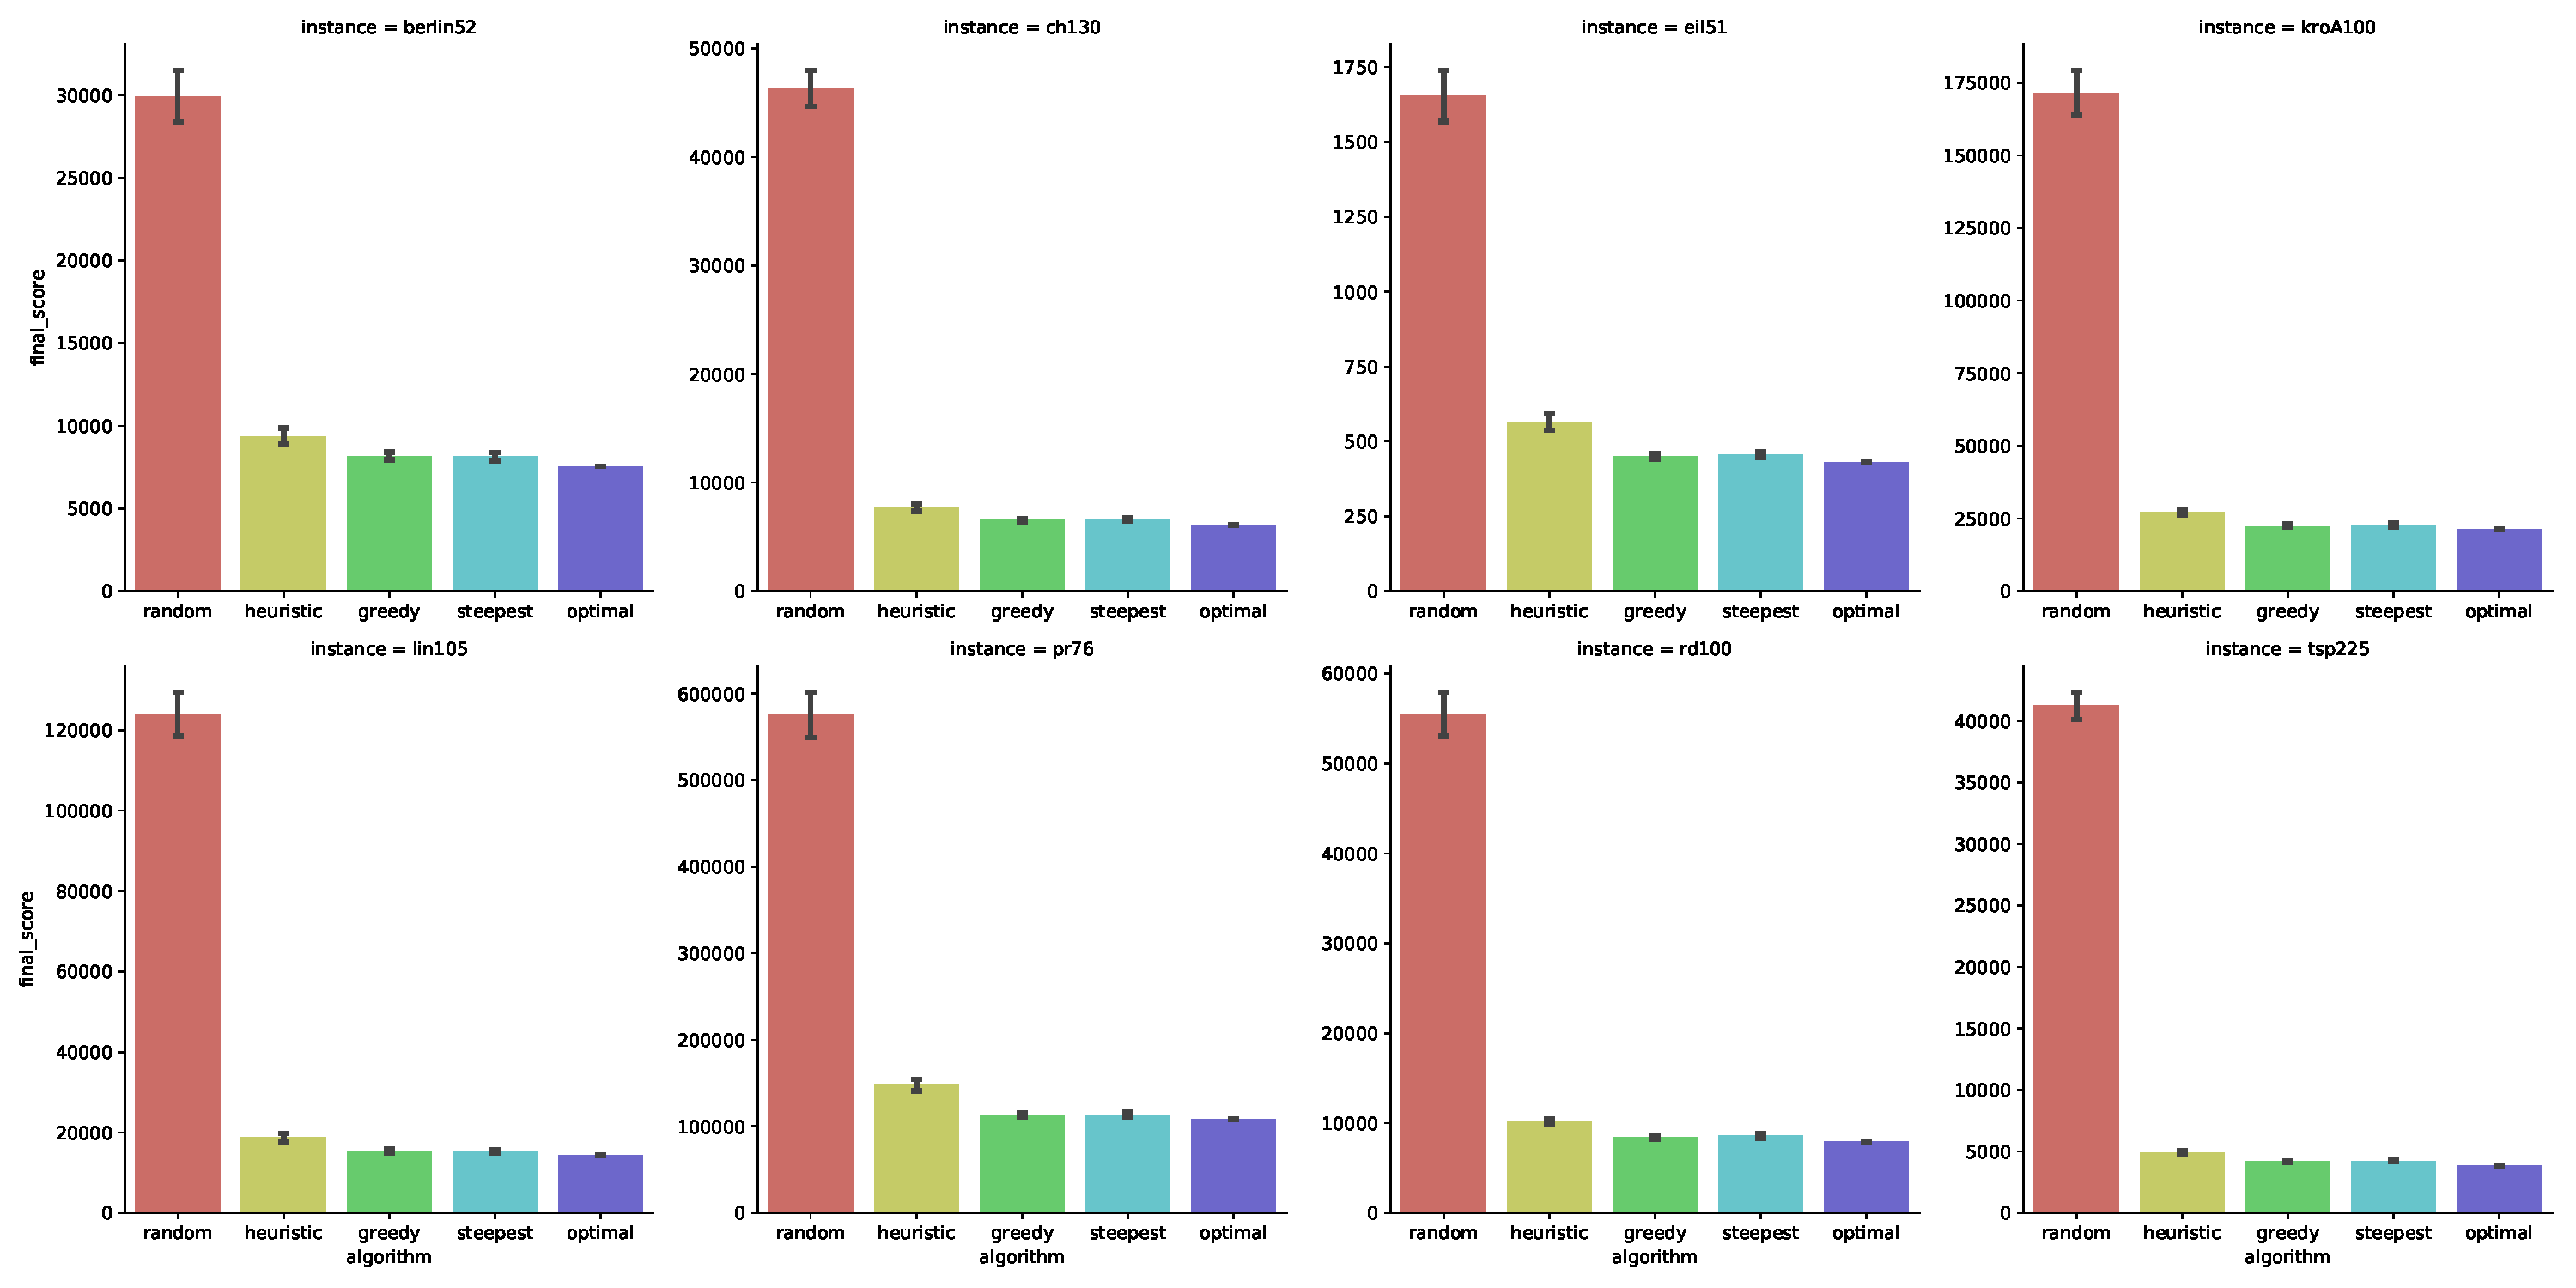
\includegraphics[width=1.0\textwidth]{graphs/score_comparison_bar_avg.pdf}
\end{center}
\caption{Porównanie średnich rozwiązań na~różnych instancjach.}
\label{fig:avg}
\end{figure}

%\begin{table}[H]
%\centering
%\begin{tabular}{ccc}%
%\hline
%\bfseries algorithm & \bfseries instance & \bfseries finalscore% specify table head
%\\ \hline
%\csvreader[head to column names]{graphs/score_comparison_bar_avg.csv}{}% use head of csv as column names
%{\\ \algorithm & \instance & \finalscore}% specify your coloumns here
%\\ \hline
%\end{tabular}
%\caption{Porównanie średnich rozwiązań na~różnych instancjach.}
%\label{tab:avg}
%\end{table}

\begin{figure}[H]
\begin{center}
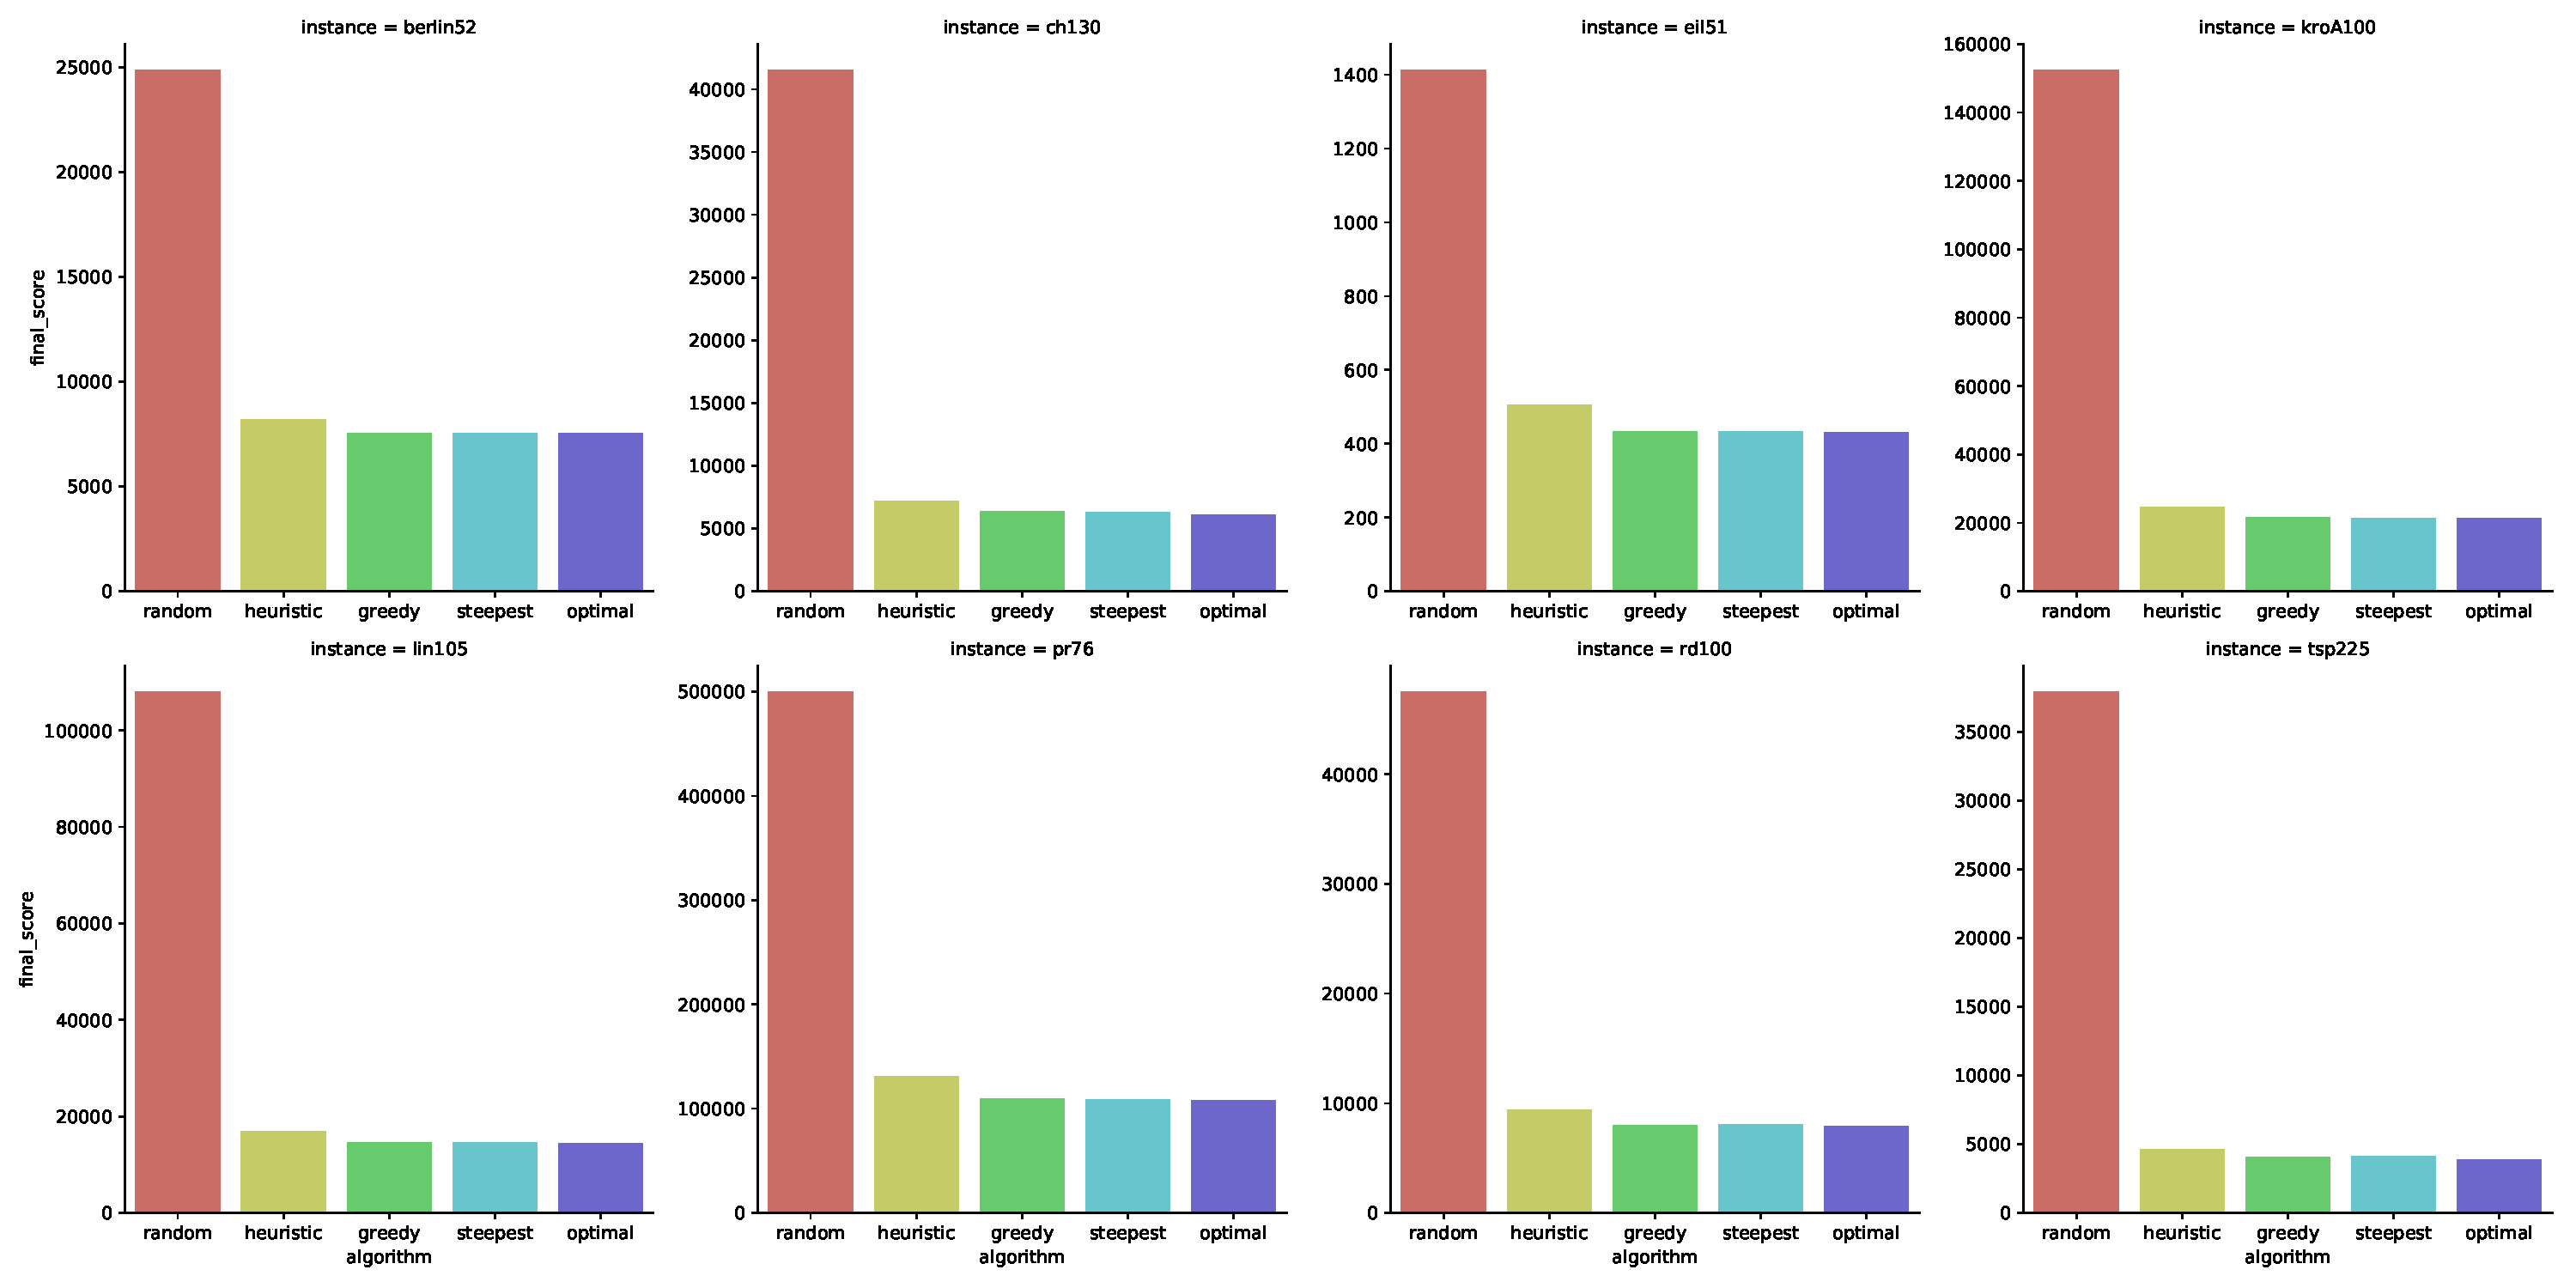
\includegraphics[width=1.0\textwidth]{graphs/score_comparison_bar_min.pdf}
\end{center}
\caption{Porównanie najlepszych znalezionych rozwiązań przez~algorytmy na~różnych instancjach.}
\label{fig:best}
\end{figure}

\begin{figure}[H]
\begin{center}
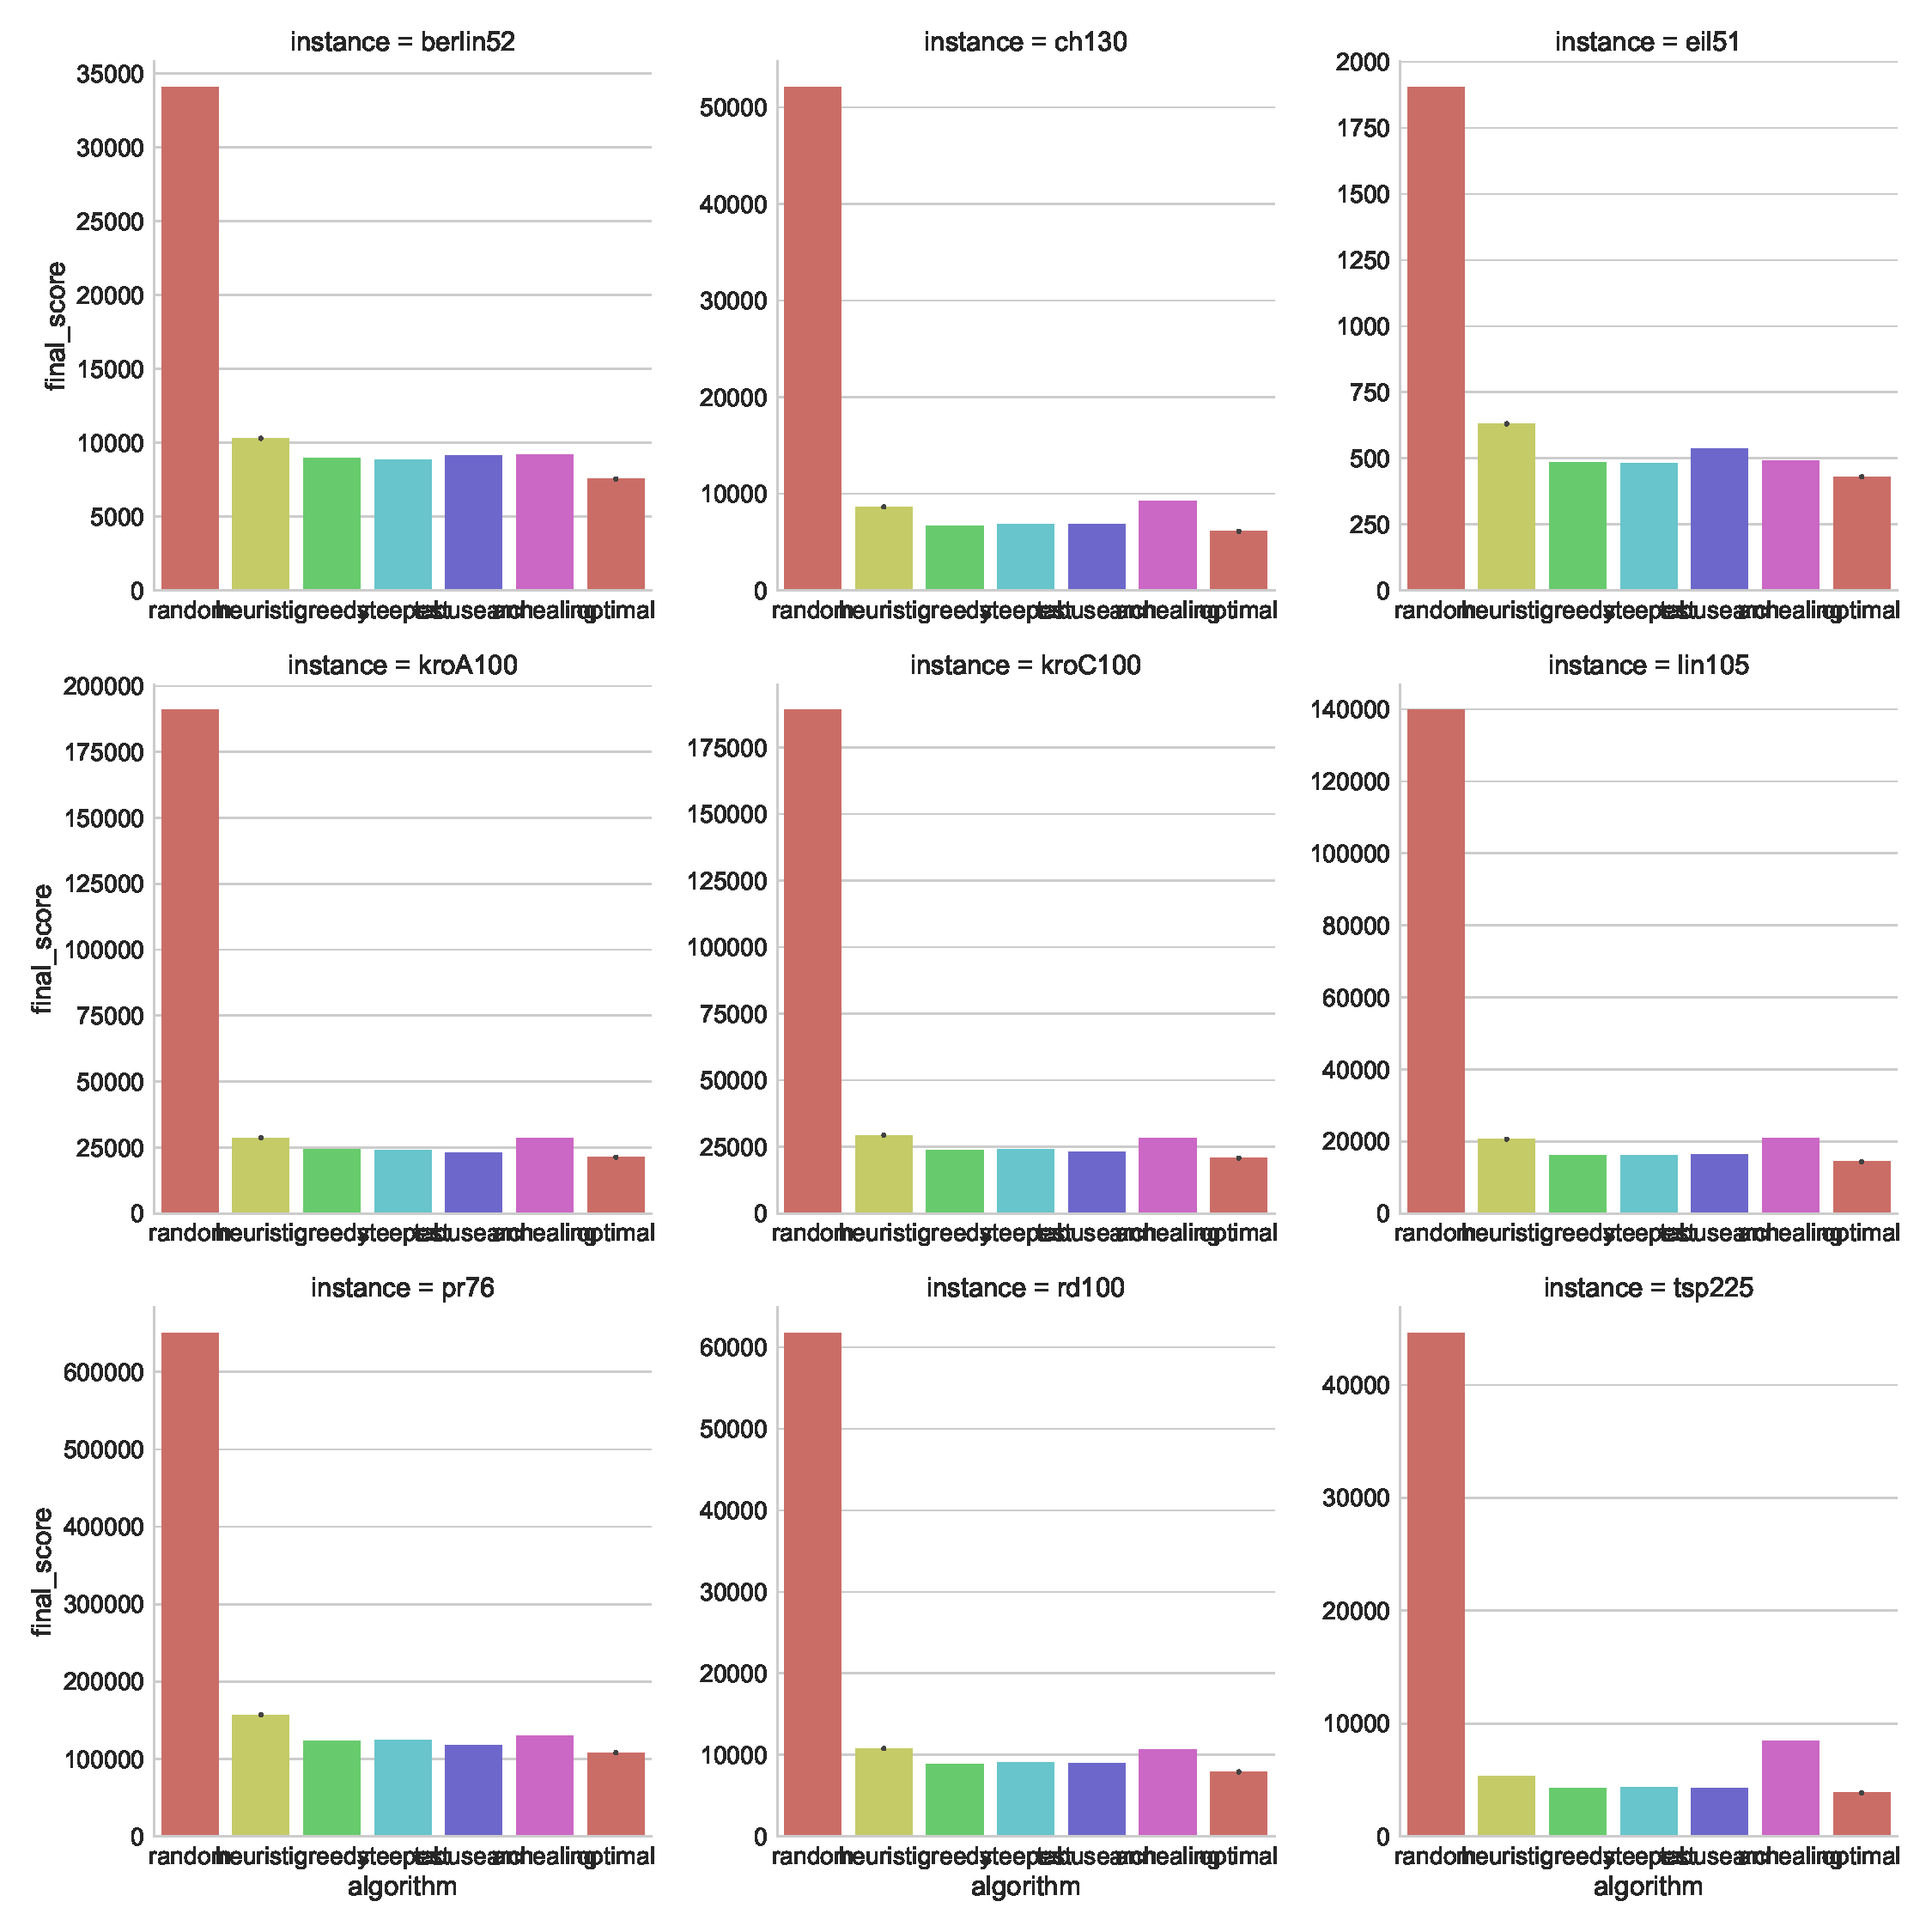
\includegraphics[width=1.0\textwidth]{graphs/score_comparison_bar_max.pdf}
\end{center}
\caption{Porównanie najgorszych znalezionych rozwiązań przez~algorytmy na~różnych instancjach.}
\label{fig:worst}
\end{figure}

\begin{figure}[H]
\begin{center}
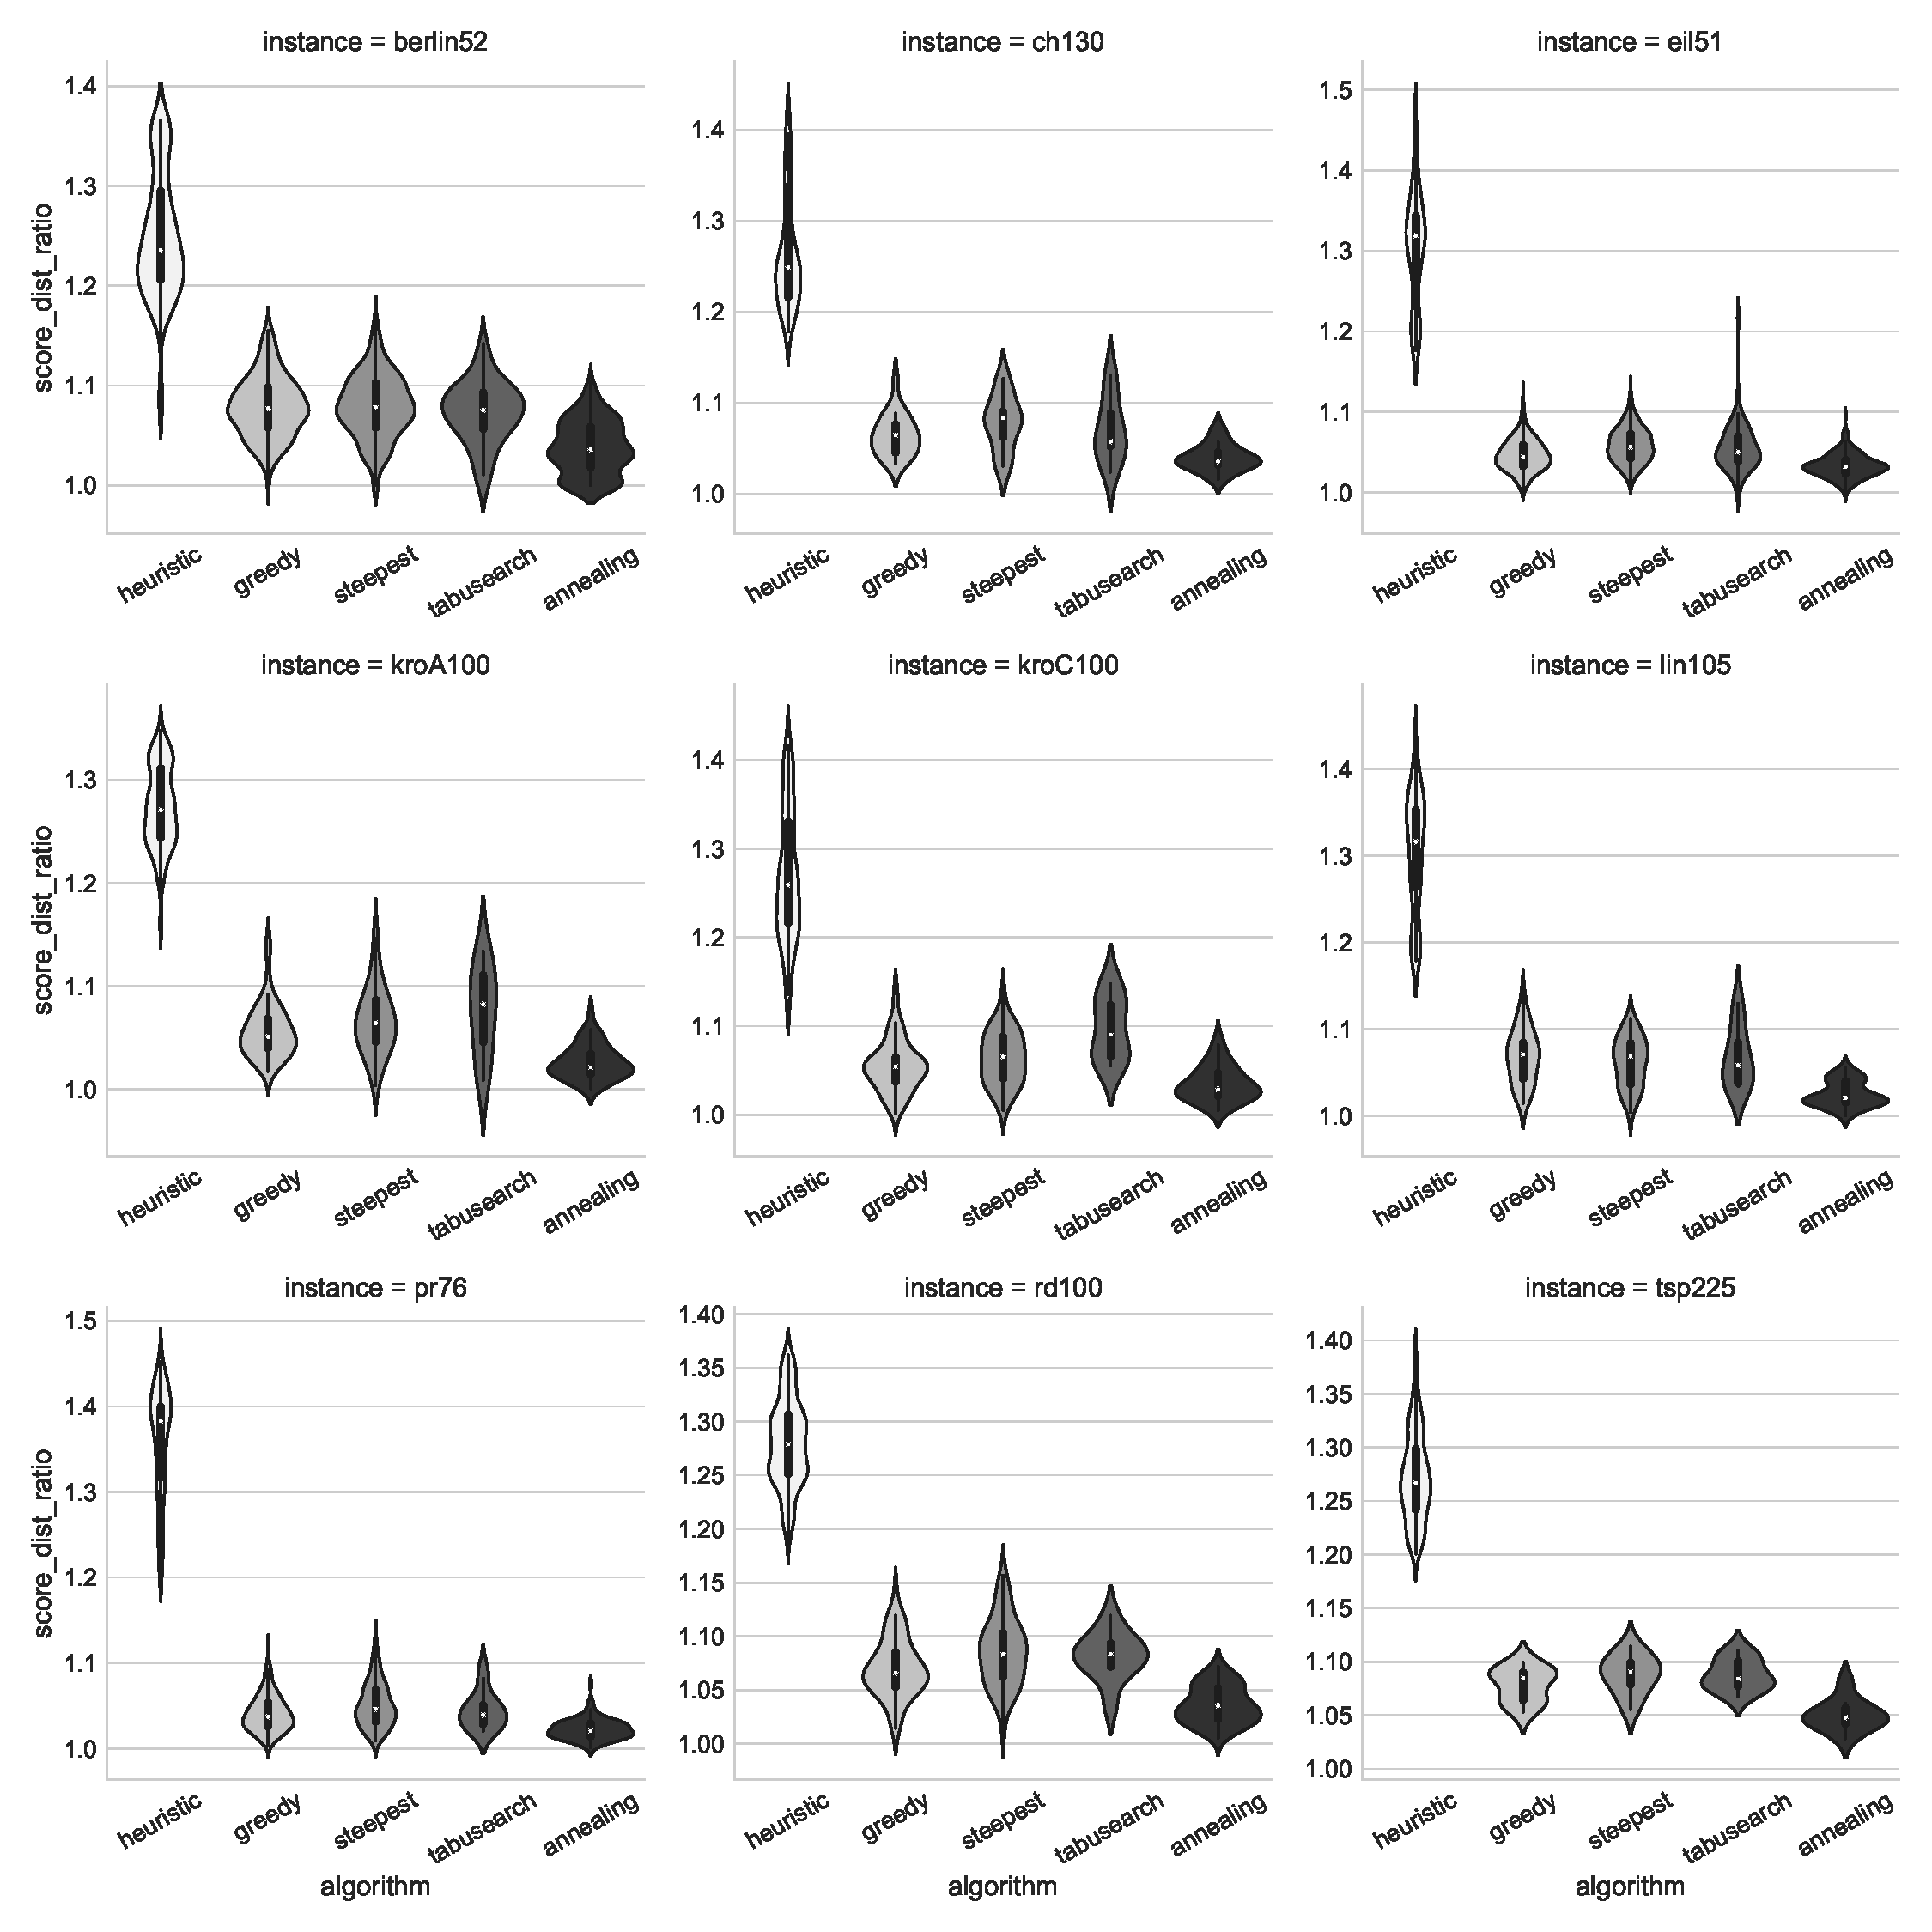
\includegraphics[width=1.0\textwidth]{graphs/score_comparison_violin.pdf}
\end{center}
\caption{Porównanie rozkładów znalezionych rozwiązań przez~algorytmy na~różnych instancjach.}
\label{fig:distribution}
\end{figure}

\subsection{Czas działania}

Algorytm losowy jest~zdecydowanie najszybszy, ponieważ sprawdza tylko jedno rozwiązanie. Podobnie heurystyka, jednak wyznaczenie przez nią~rozwiązania zajmuje trochę więcej czasu. Greedy i~Steepest przeszukują przestrzeń rozwiązań, dopóki nie~mogą już~bardziej poprawić wyniku, przez co~trwają zdecydowanie najdłużej. Przeważnie obliczenia Steepesta zajmują więcej czasu, niż~wykonanie algorytmu Greedy. Na~rys.~\ref{fig:time} można~też~zauważyć, że~pojedyncze wykonania trwają znacznie dłużej od~pozostałych --- szczególnie jest~to~widoczne przy~instancji berlin52.

\begin{figure}[H]
\begin{center}
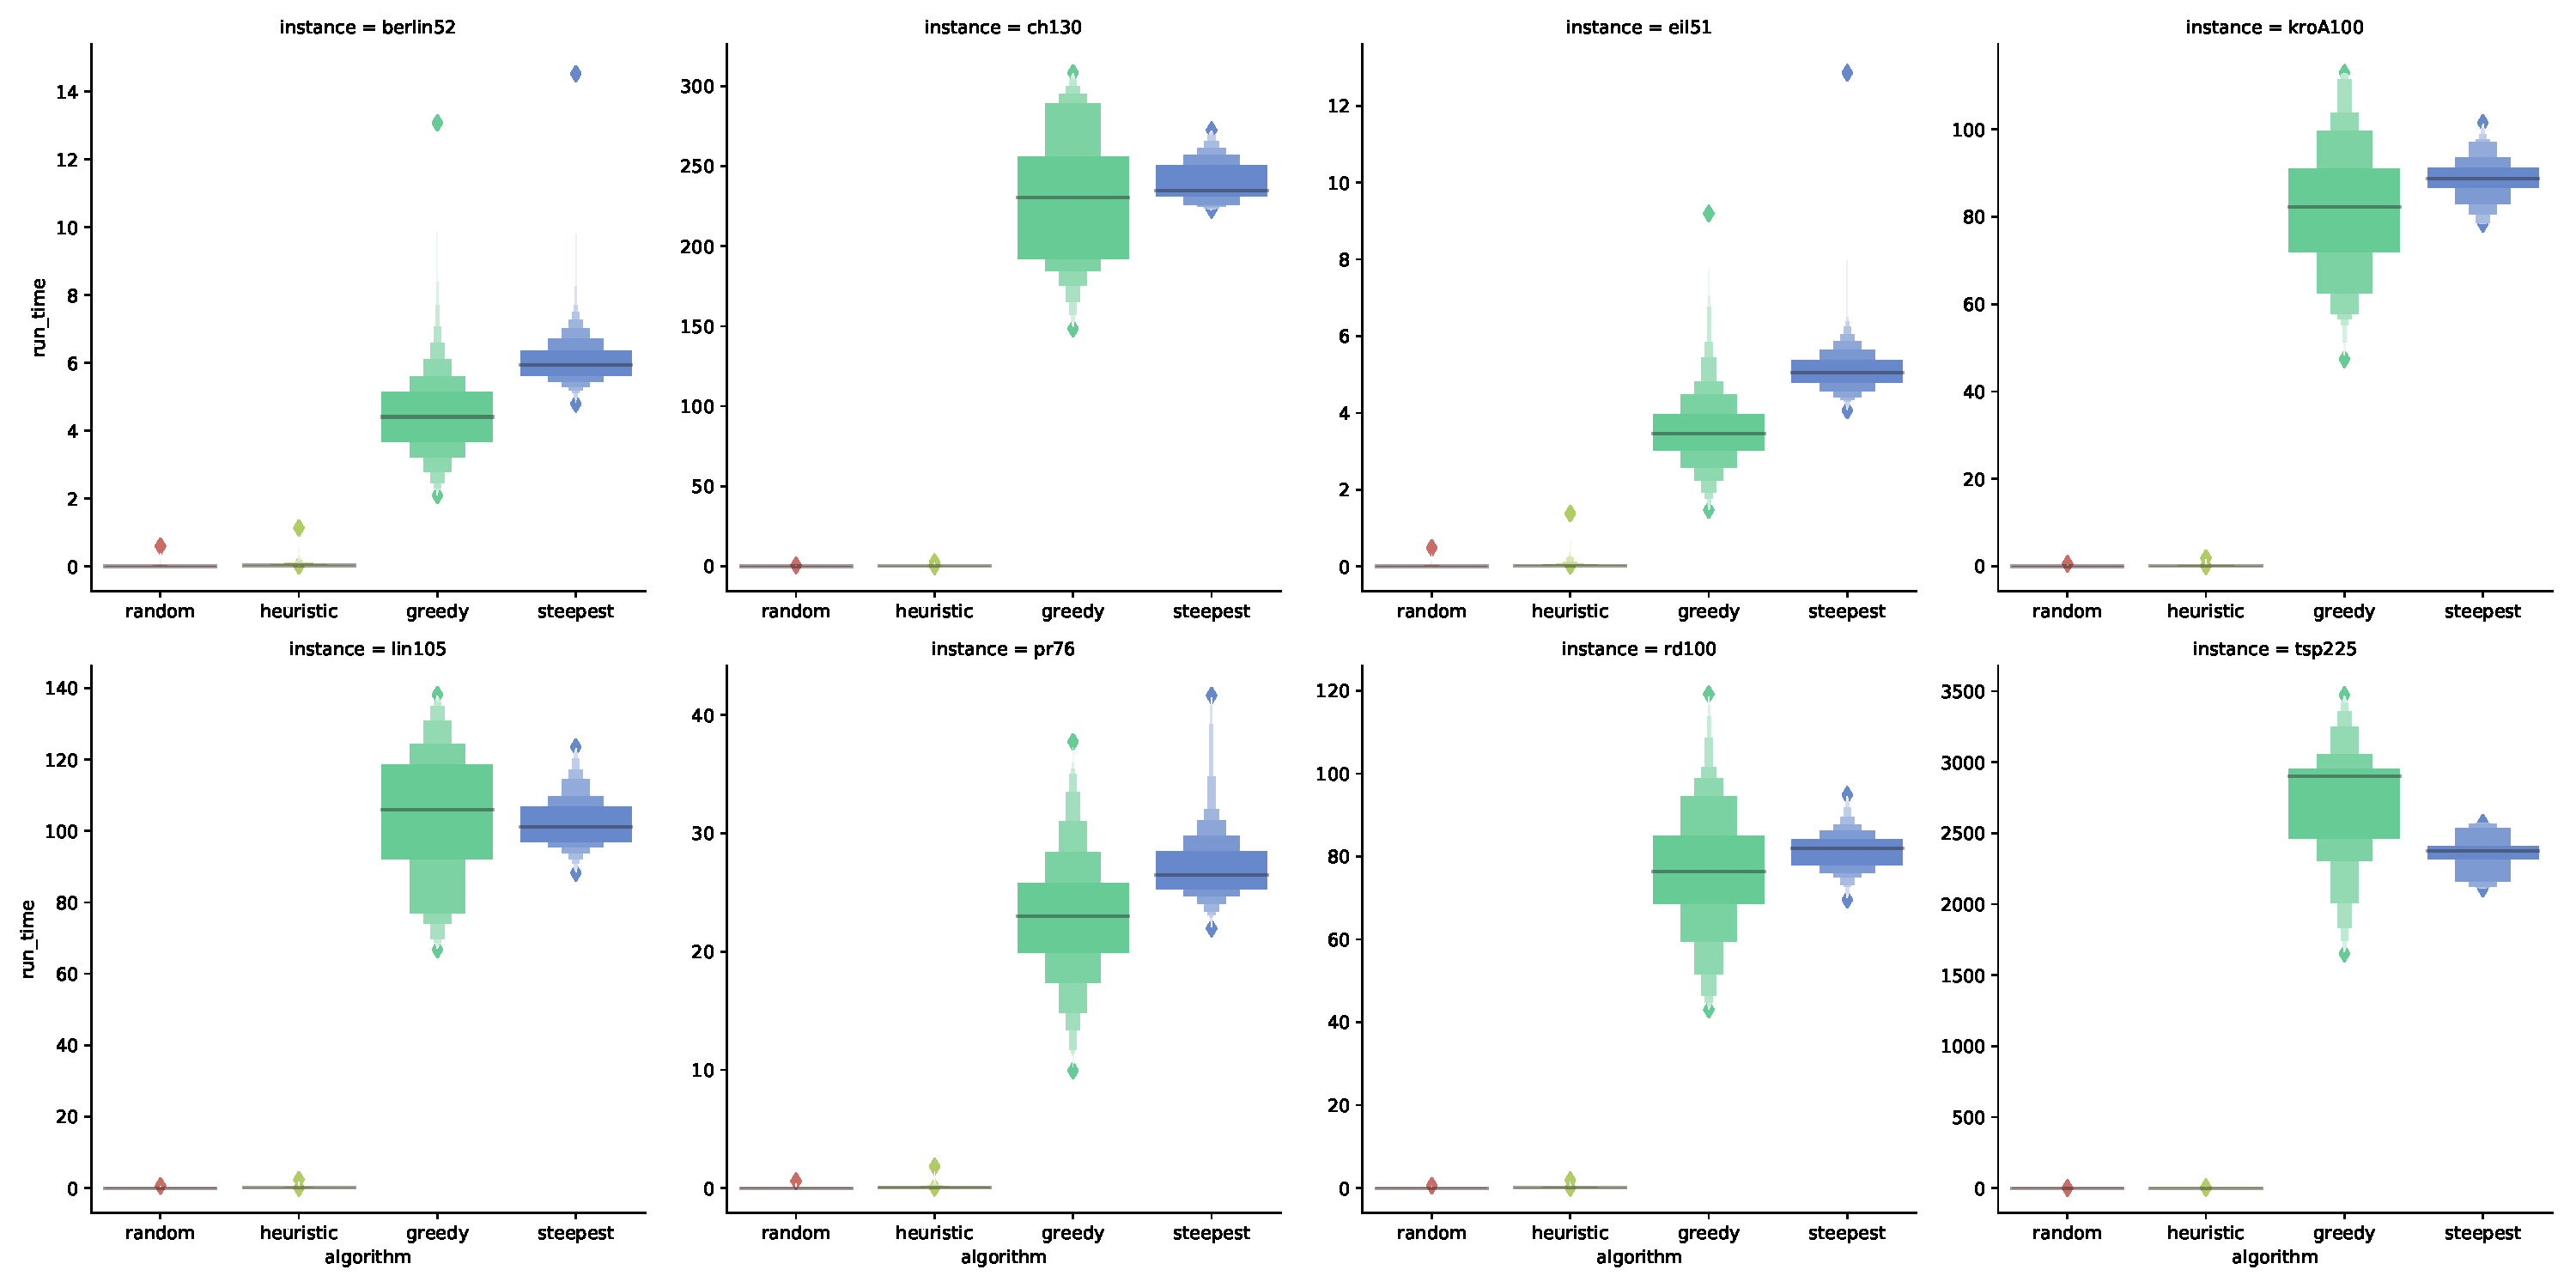
\includegraphics[width=1.0\textwidth]{graphs/time_comparison_letval.pdf}
\end{center}
\caption{Porównanie czasu działania algorytmów na~poszczególnych instancjach.}
\label{fig:time}
\end{figure}

\subsection{Efektywność algorytmów}

\subsubsection{Wybrana miara}

Aby porównać algorytmy pod~względem jakości, można to~zrobić przez zdefiniowanie kosztu czasowego, jaki~trzeba ponieść, aby~uzyskać dane rozwiązanie. Czyli należy policzyć iloraz $cost = time / result$, co~jest~przedstawione na~rys.~\ref{fig:cost}. Natomiast efektywnością algorytmu jest~odwrotność kosztu, która została przedstawiona na~rys.~\ref{fig:quality}.

\subsubsection{Wyniki}

Z~wykresów~\ref{fig:cost} i~\ref{fig:quality} można by~wyciągnąć wniosek, że~najefektywniejszym algorytmem jest~algorytm losowy, ponieważ zajmuje najmniej czasu. Takie wyniki są~jednak konsekwencją tego, że~przy każdy krok algorytmu przeszukiwania lokalnego jest~dość kosztowny, ponieważ przegląda się wiele rozwiązań, a~rozwiązanie jest~poprawiane nieznacznie (zgodnie z~założeniem algorytmów przeszukiwania lokalnego, że~funkcja celu sąsiadów niewiele się różni). Podobnie przy heurystyce --- nawet złożoność $\theta(n^2)$ nie~gwarantuje ulepszenia rozwiązania n-krotnie, a~jedynie kilkukrotnie, więc~koszt algorytmu jest~stosunkowo wysoki.

Na~wykresie kosztu widać również, że~Greedy jest~kosztowniejszy od~Steepesta, ponieważ daje zbliżone rozwiązania w~dłuższym czasie.

\begin{figure}[H]
\begin{center}
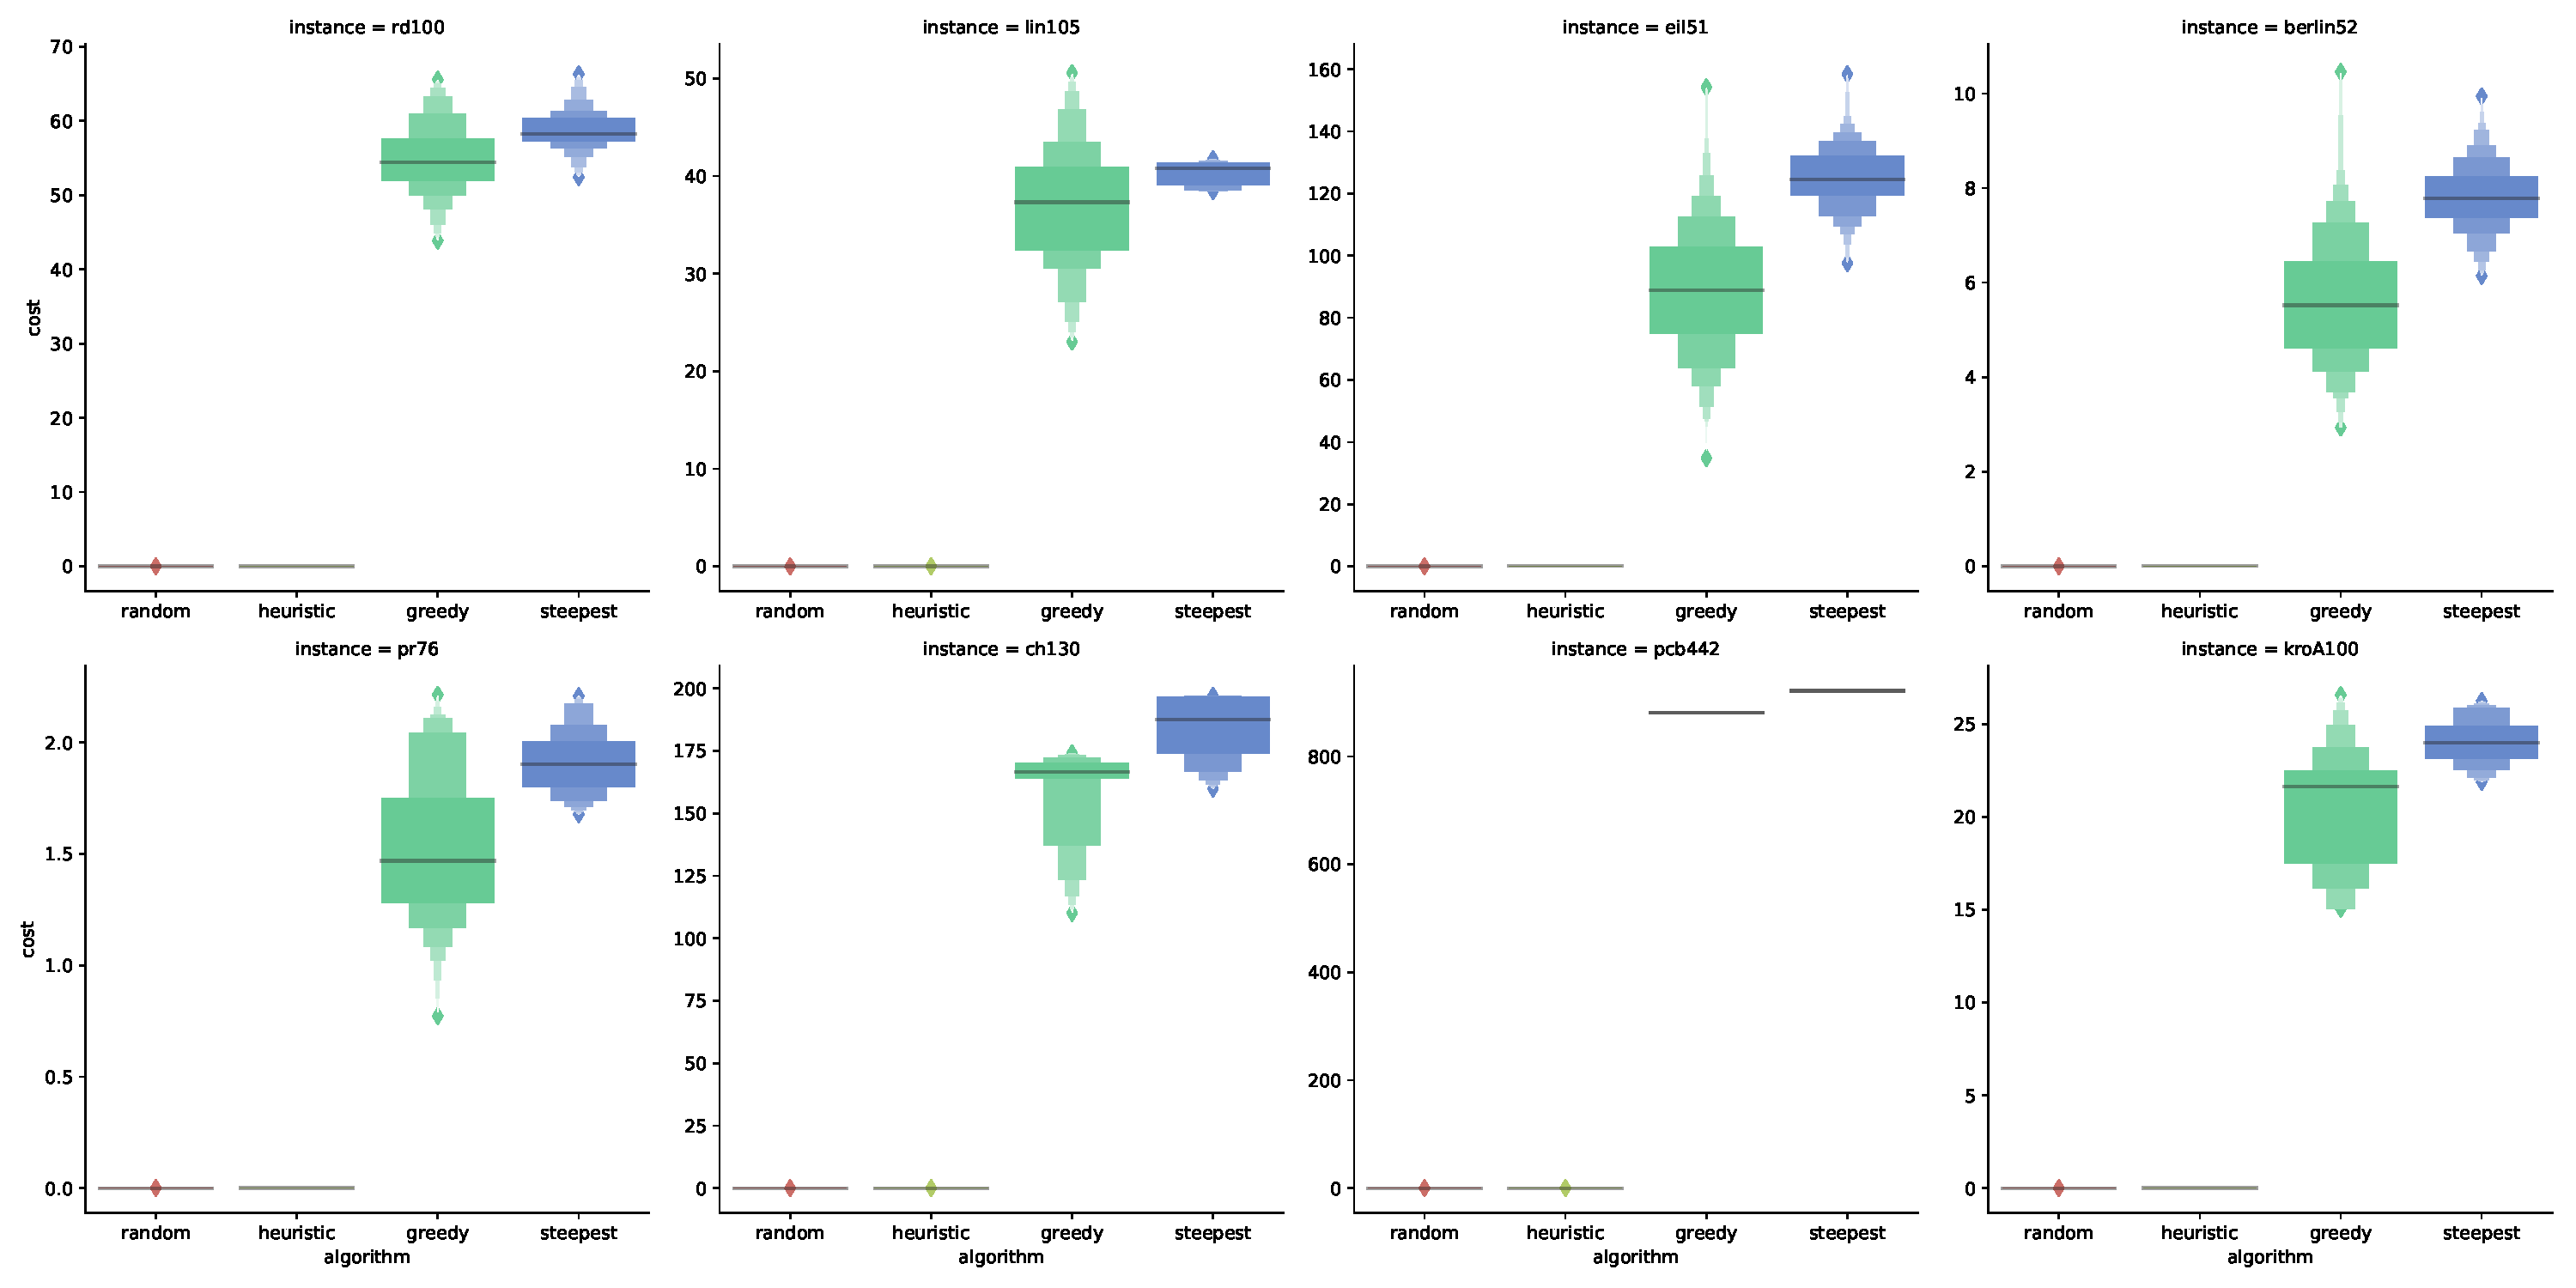
\includegraphics[width=1.0\textwidth]{graphs/cost_comparison_letval.pdf}
\end{center}
\caption{Porównanie kosztów algorytmów na~poszczególnych instancjach.}
\label{fig:cost}
\end{figure}

\begin{figure}[H]
\begin{center}
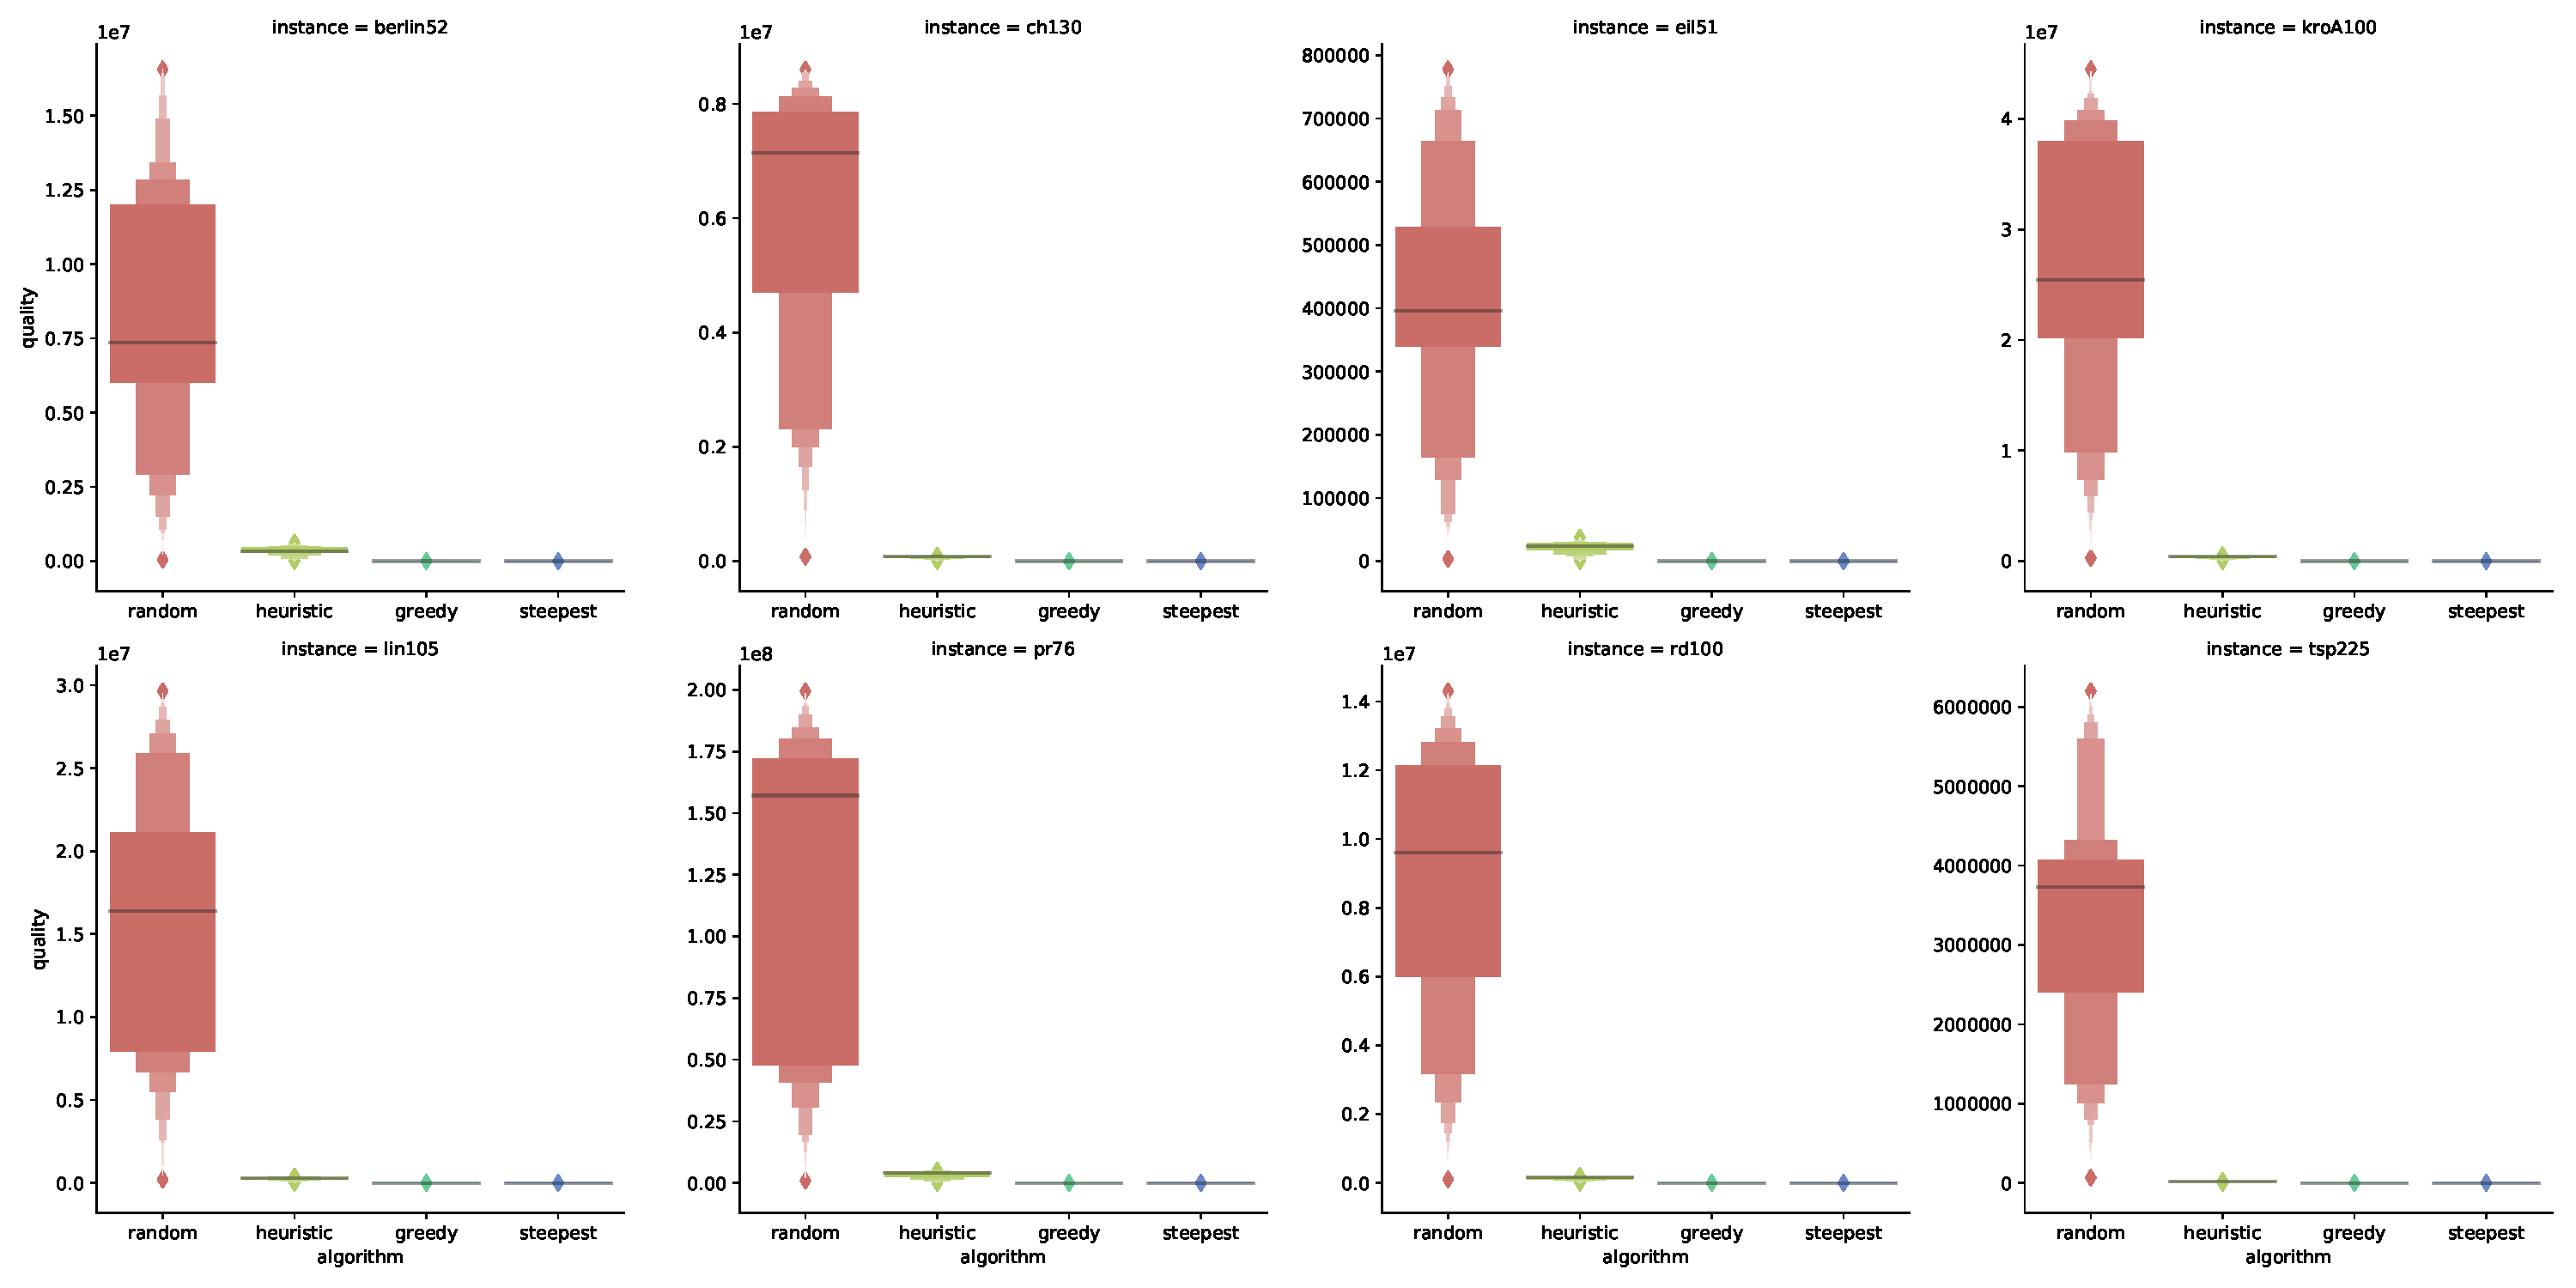
\includegraphics[width=1.0\textwidth]{graphs/quality_comparison_letval.pdf}
\end{center}
\caption{Porównanie efektywności algorytmów na~poszczególnych instancjach.}
\label{fig:quality}
\end{figure}

\subsection{Liczba kroków algorytmów lokalnego przeszukiwania}

Wykres~\ref{fig:steps} przedstawia liczbę kroków wykonanych przez algorytmy lokalnego przeszukiwania. Widać, że~Greedy wykonuje ich kilkakrotnie więcej niż~Steepest, a~także, że~liczba wykonanych kroków przez ten~algorytm jest~dużo bardziej zróżnicowana, w~zależności od~przypadku startowego. Jest~to~spowodowane tym, że~algorytm Steepest we~wcześniejszym kroku osiąga lokalnie najlepsze rozwiązanie, ponieważ za~każdym razem wybiera to, które~najbardziej poprawia wynik z~całego sąsiedztwa.

\begin{figure}[H]
\begin{center}
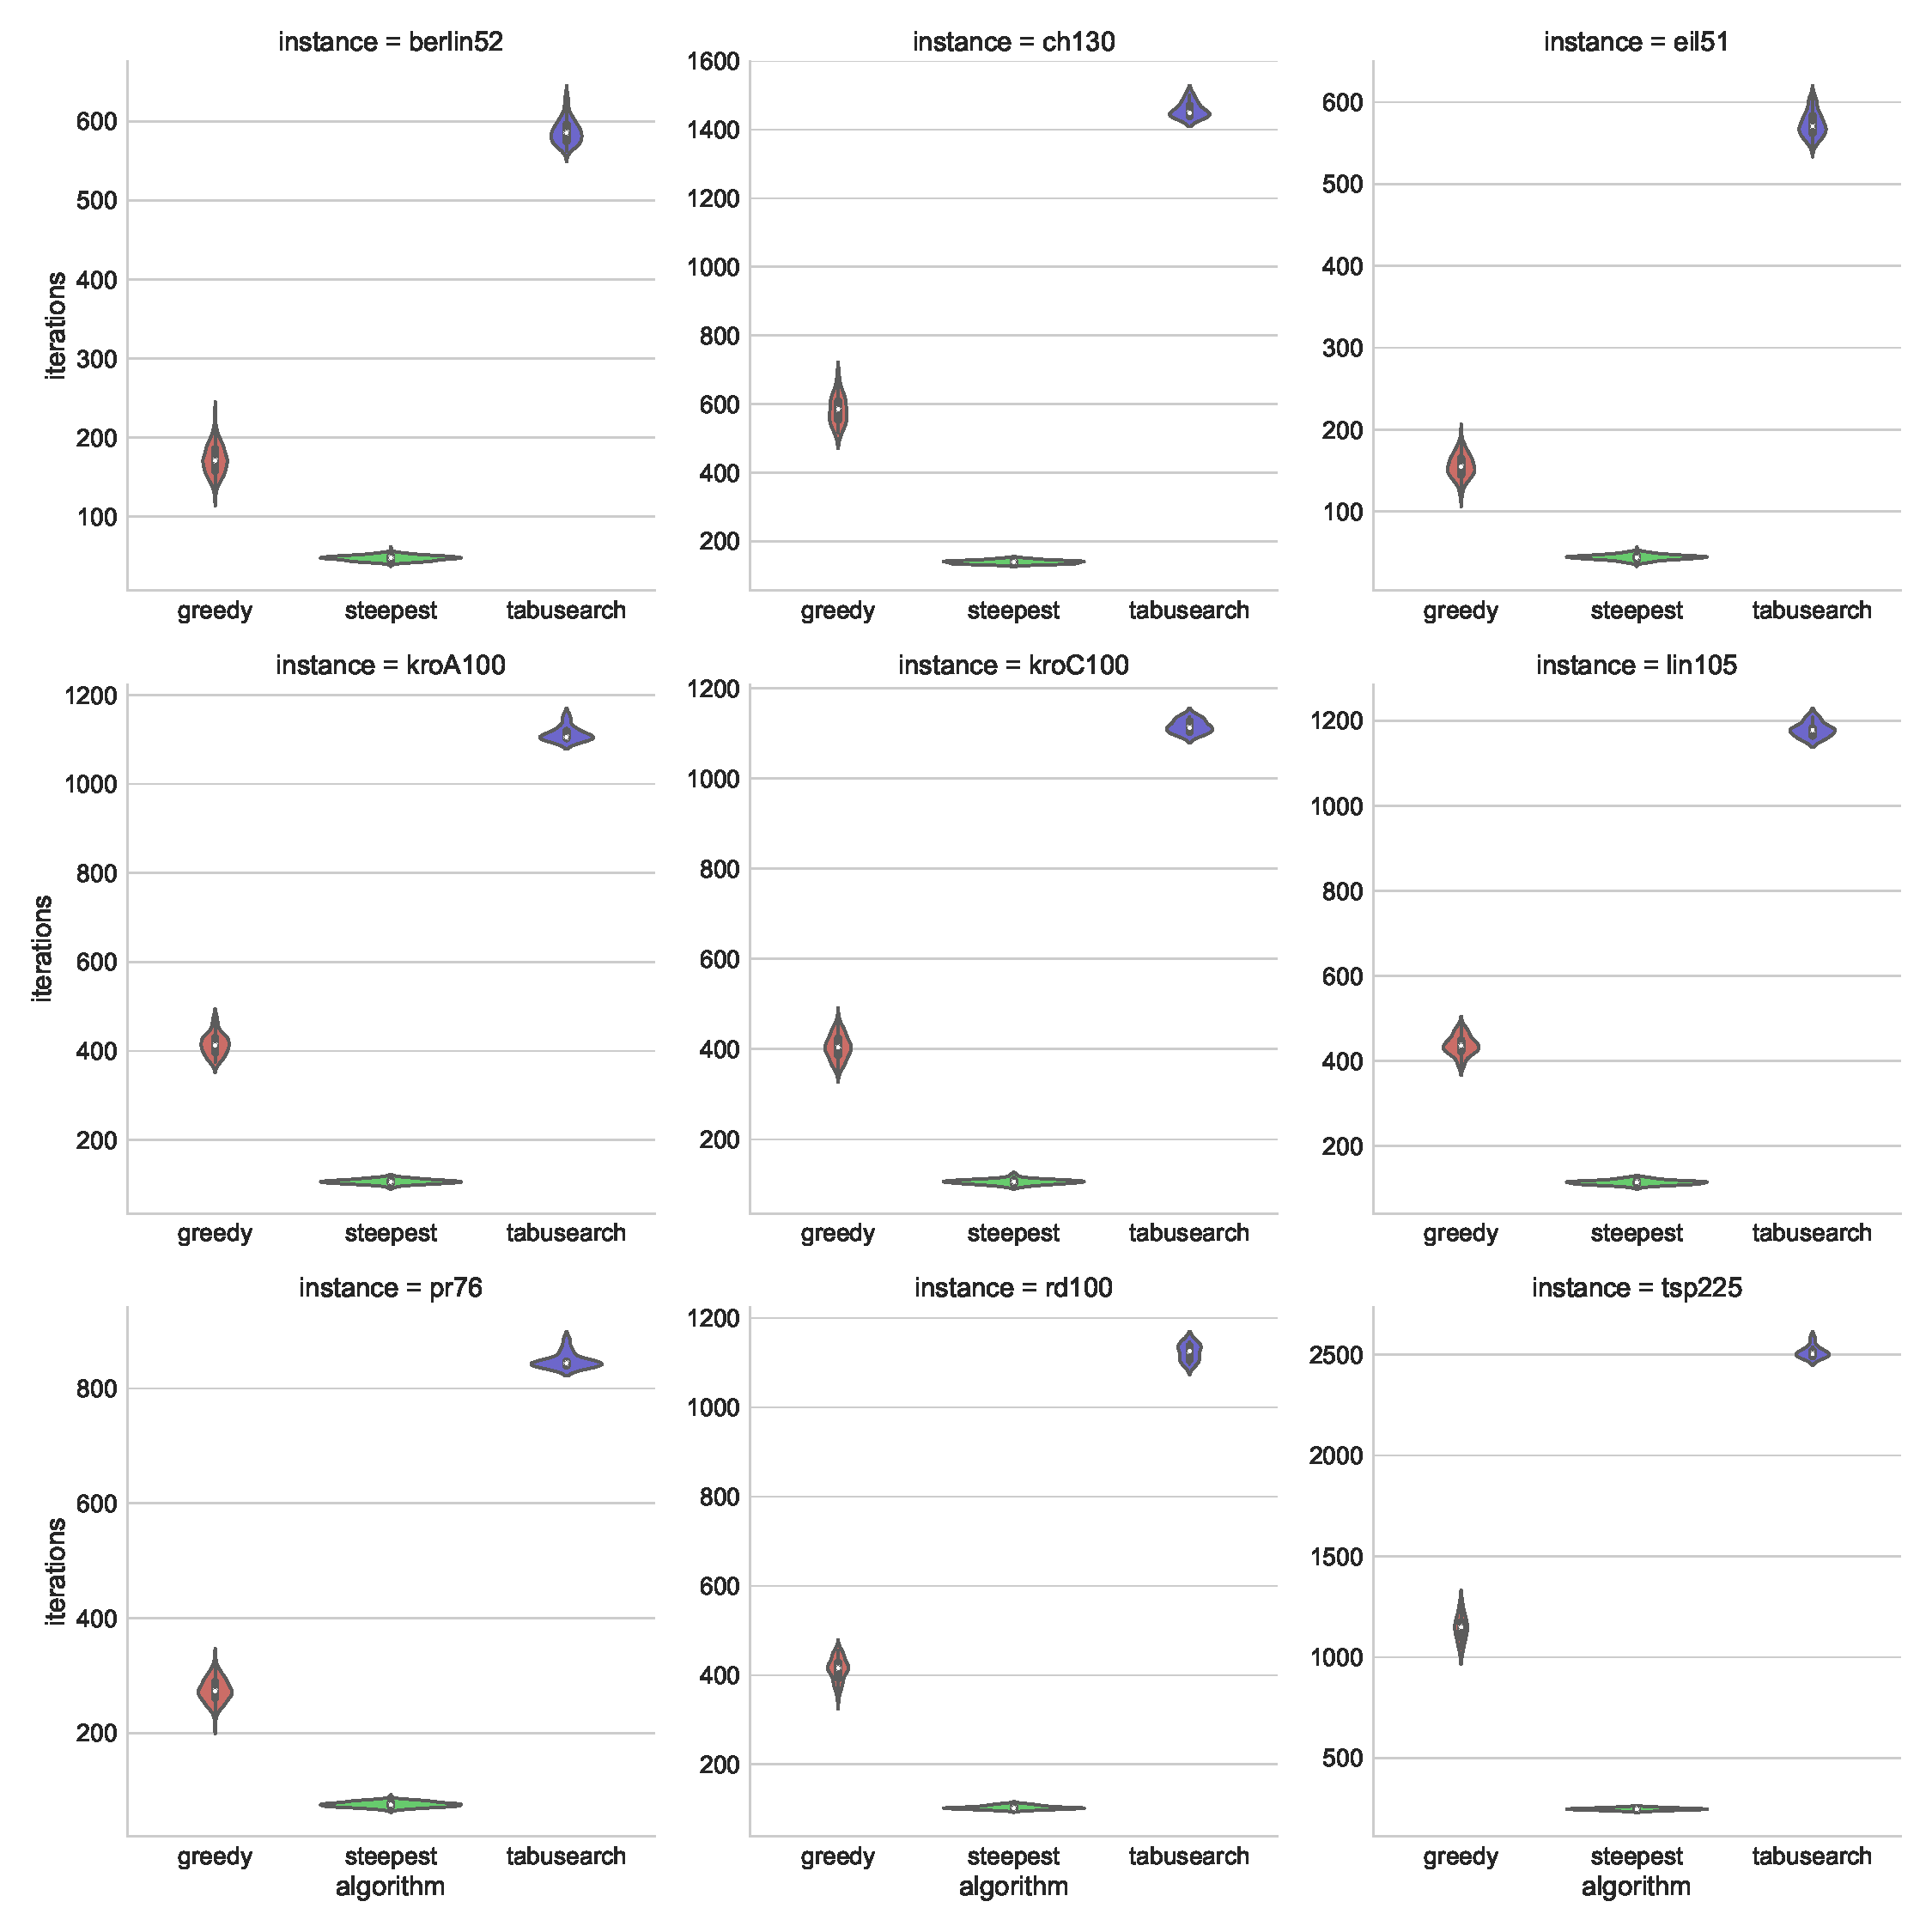
\includegraphics[width=1.0\textwidth]{graphs/iterations_comparison_violin.pdf}
\end{center}
\caption{Porównanie algorytmów Greedy Search i~Steepest pod~względem liczby kroków do~zatrzymania.}
\label{fig:steps}
\end{figure}

\subsection{Średnia liczba przeszukanych rozwiązań}

Na~wykresie \ref{fig:nsol} jest~przedstawiona liczba rozwiązań przeszukiwanych przez~oba rozważane algorytmy lokalnego przeszukiwania. Można na~nim~zauważyć, że~średnio Steepest przeszukuje większą przestrzeń, choć~zdarzają się wykonania algorytmu Greedy, które~sprawdzają większą liczbę rozwiązań. Jest to~o~tyle ciekawe, że~Steepest wykonuje mniej kroków, niż~Greedy, a~i~tak aby~je~wykonać, przegląda więcej rozwiązań. Co~ciekawe, ta~tendencja jest~odmienna dla~największej instancji, podobnie~też, czas działania algorytmu Greedy dla~niej jest~większy od~Steepesta.

\begin{figure}[H]
\begin{center}
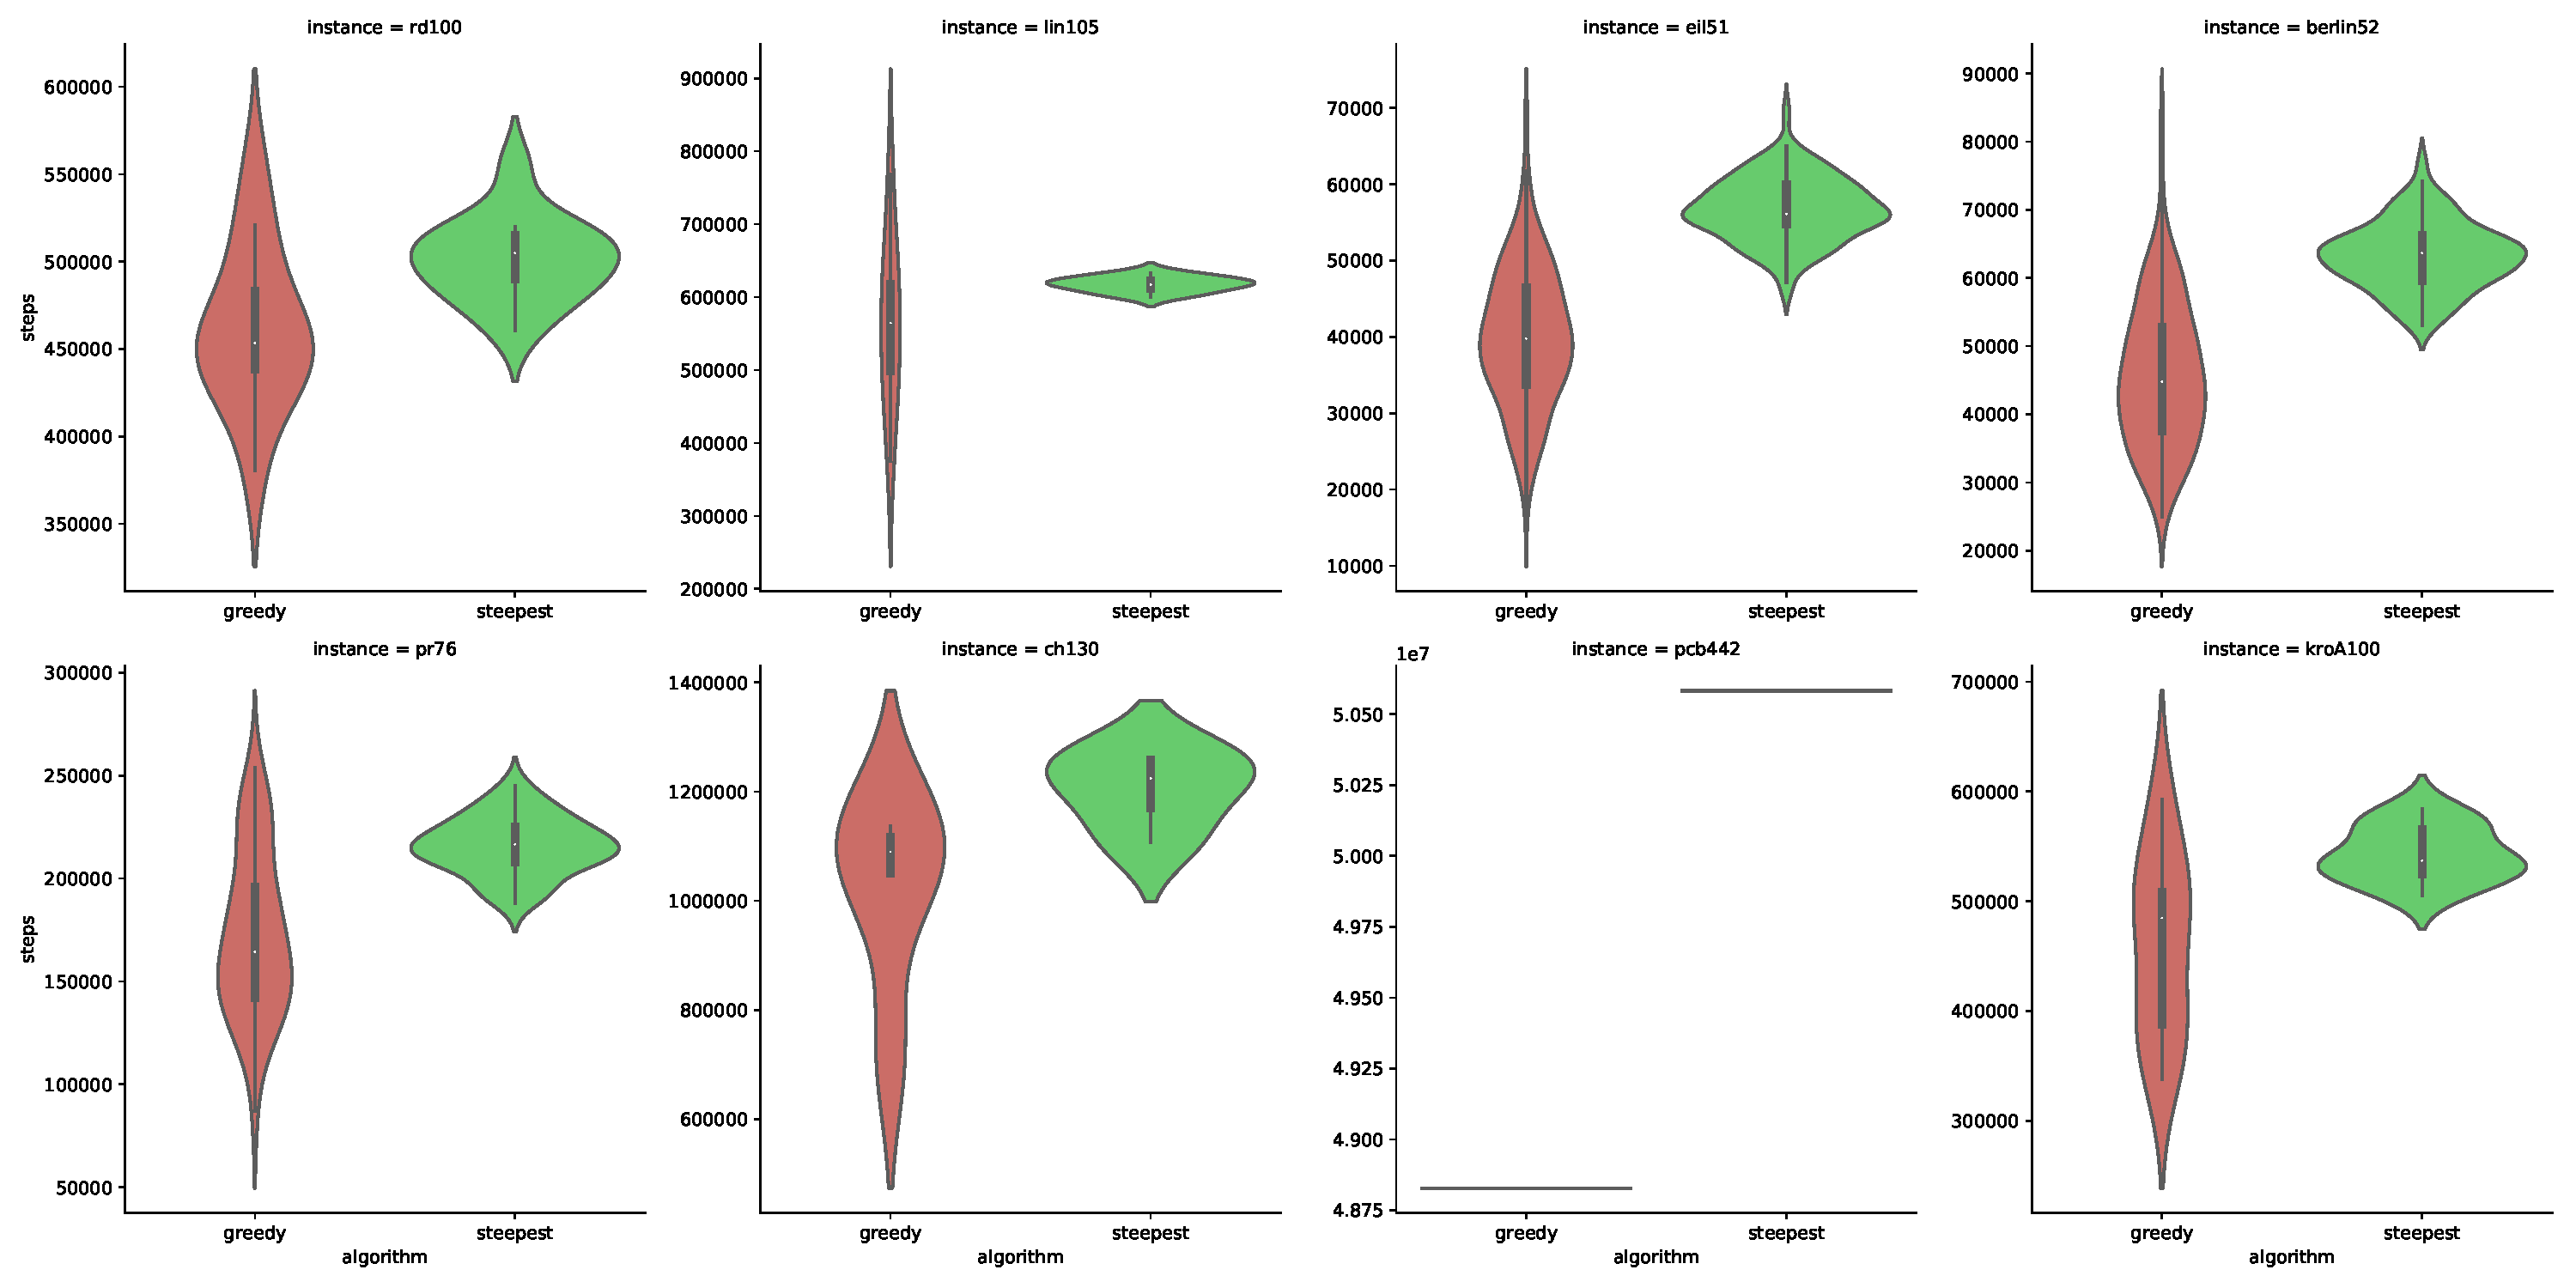
\includegraphics[width=1.0\textwidth]{graphs/steps_comparison_violin.pdf}
\end{center}
\caption{Porównanie algorytmów Greedy Search i~Steepest pod~względem liczby przeszukanych rozwiązań.}
\label{fig:nsol}
\end{figure}

\subsection{Przeszukiwanie lokalne}

\subsubsection{Jakość rozwiązania początkowego a końcowego}

Badając zależność między rozwiązaniem początkowym, a~końcowym, nie~udało nam się zaobserwować związku na~wykresie punktowym \ref{fig:diff_point}. Punkty są~bardzo rozrzucone i~nie~daje się ich~odpowiednio pogrupować. Na~wykresie skrzypcowym~\ref{fig:diff} zostały przedstawione rozwiązania początkowe i~końcowe dla~obu~algorytmów. Widać, że~są~wyraźnie od~siebie oddalone i~zgrupowane w~osobne chmury. Można zatem przypuszczać, że~jakość rozwiązania końcowego nie~zależy od~jakości rozwiązania początkowego.

\begin{figure}[H]
\begin{center}
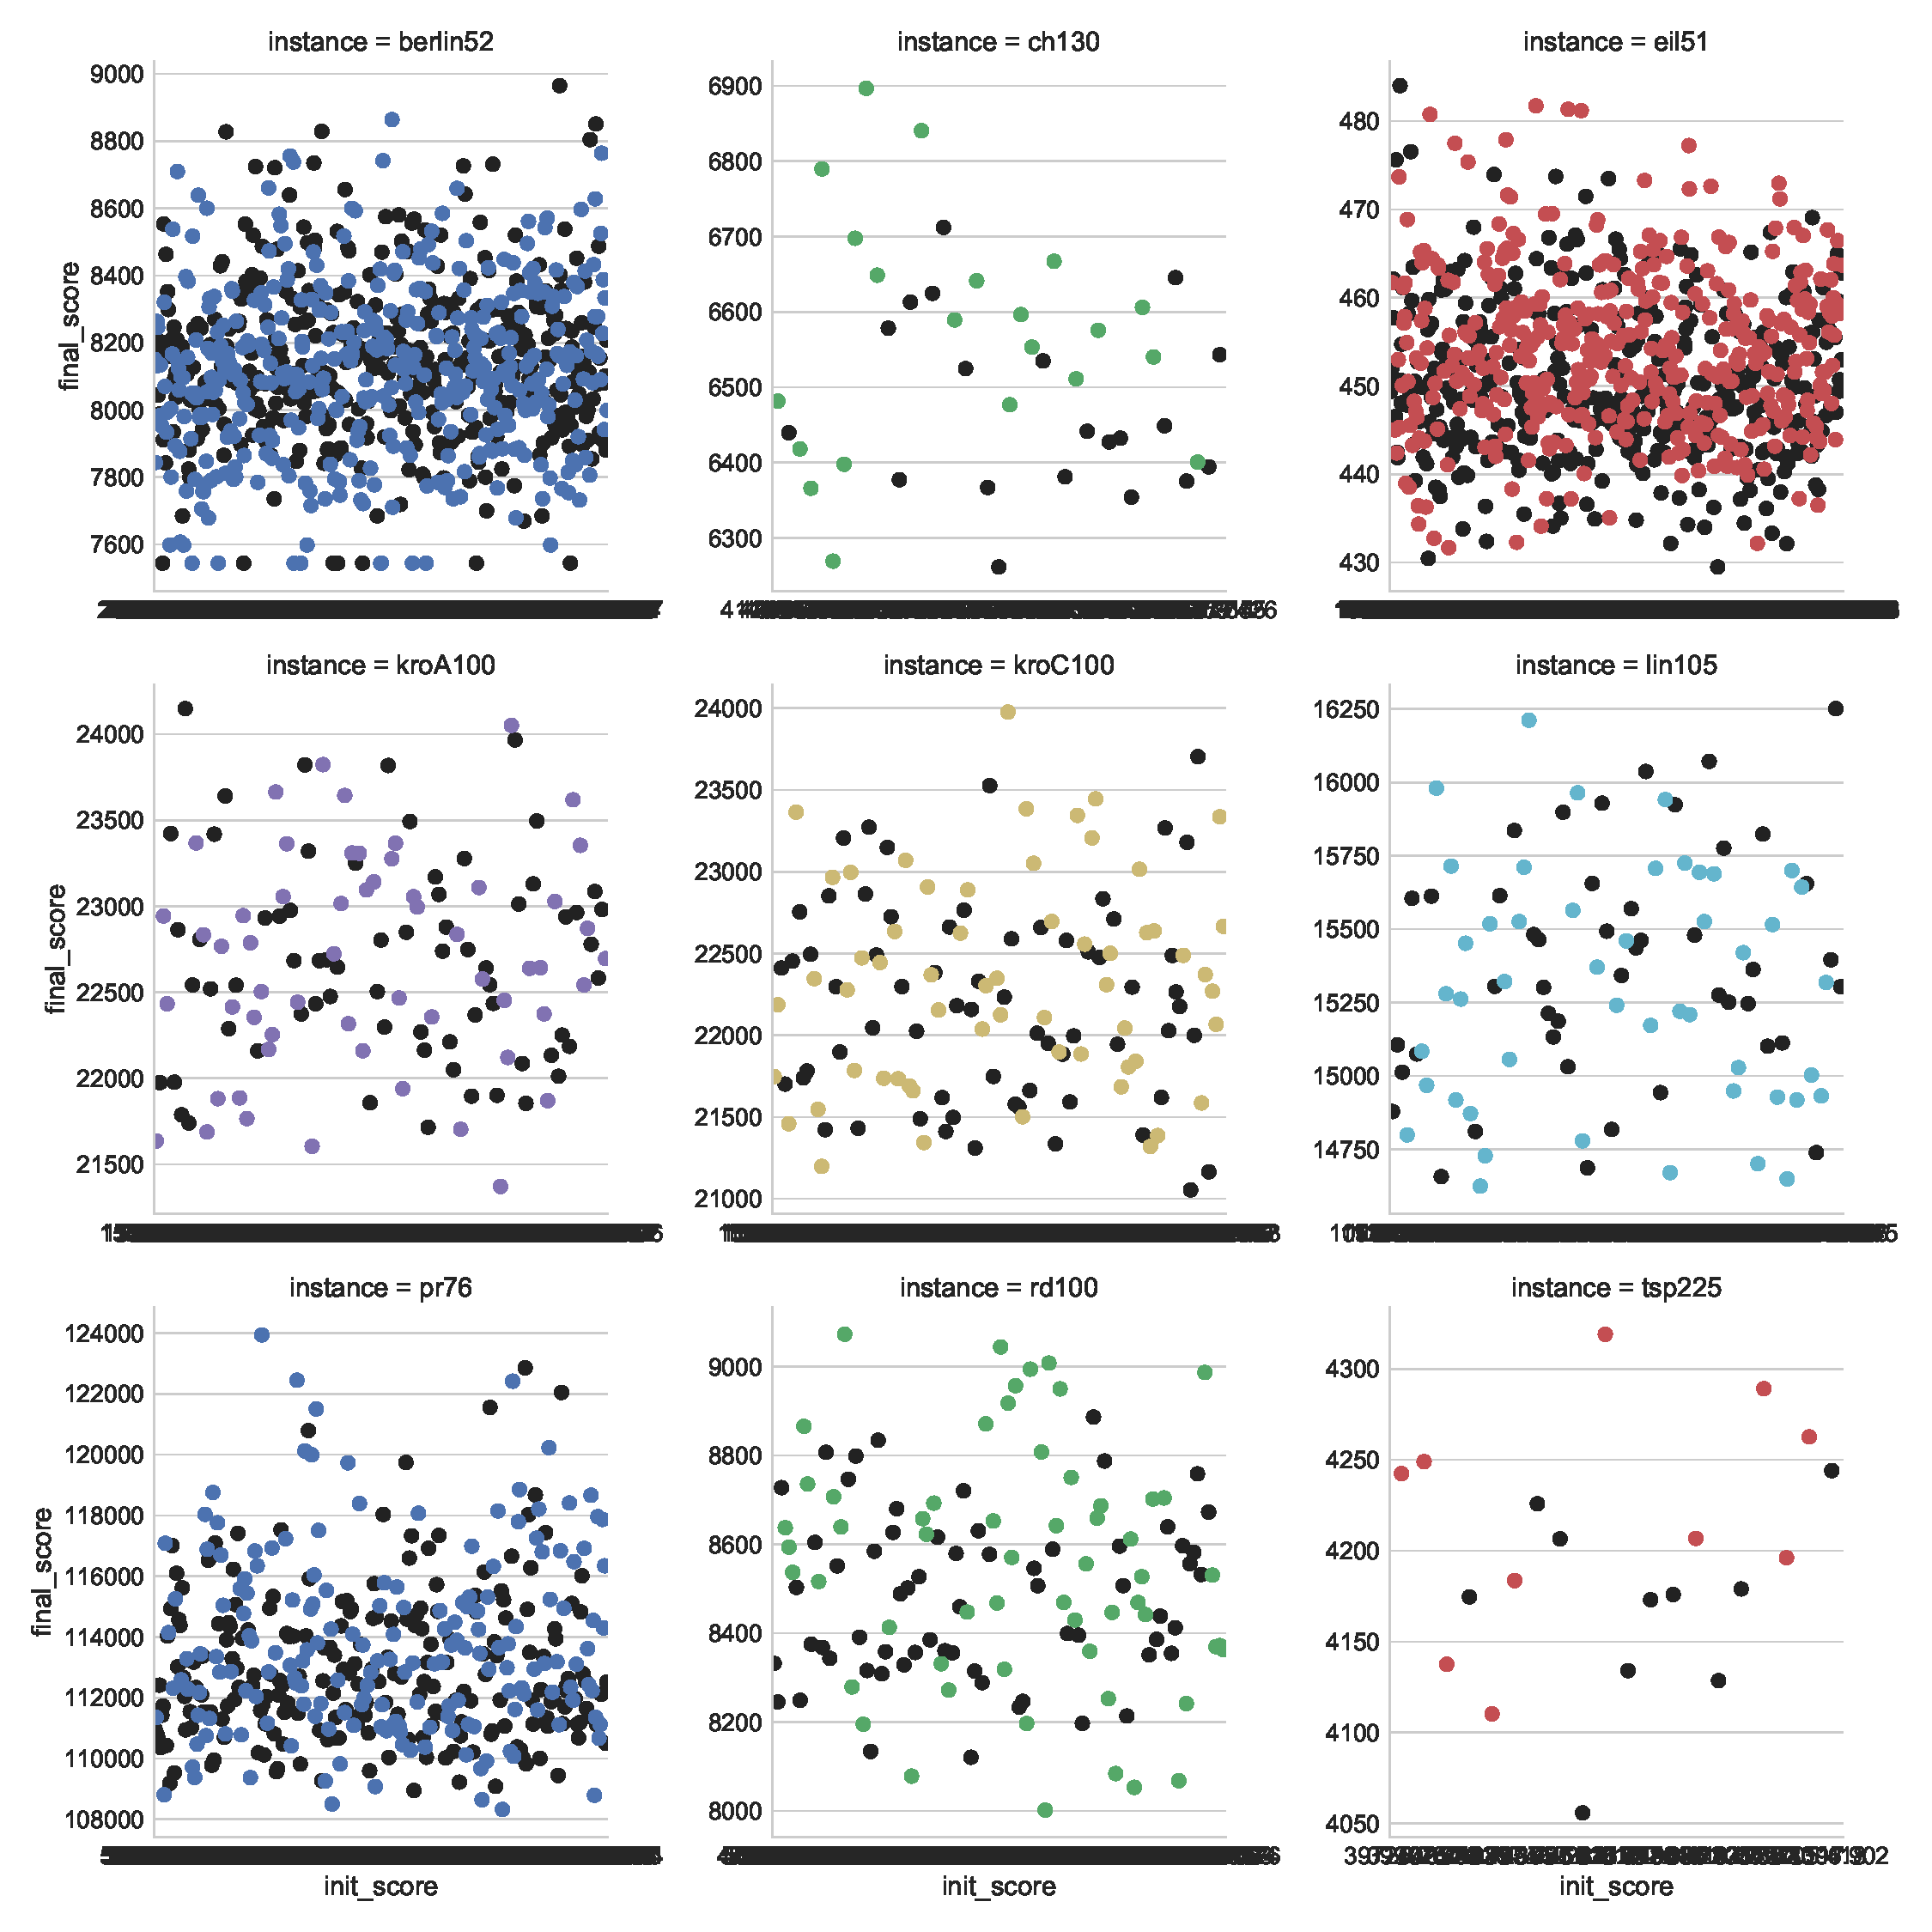
\includegraphics[width=1.0\textwidth]{graphs/init_vs_final_score_point.pdf}
\end{center}
\caption{Porównanie jakości rozwiązań początkowych i~końcowych przez~algorytmy Greedy Search i~Steepest przedstawione na wykresie punktowym.}
\label{fig:diff_point}
\end{figure}

\begin{figure}[H]
\begin{center}
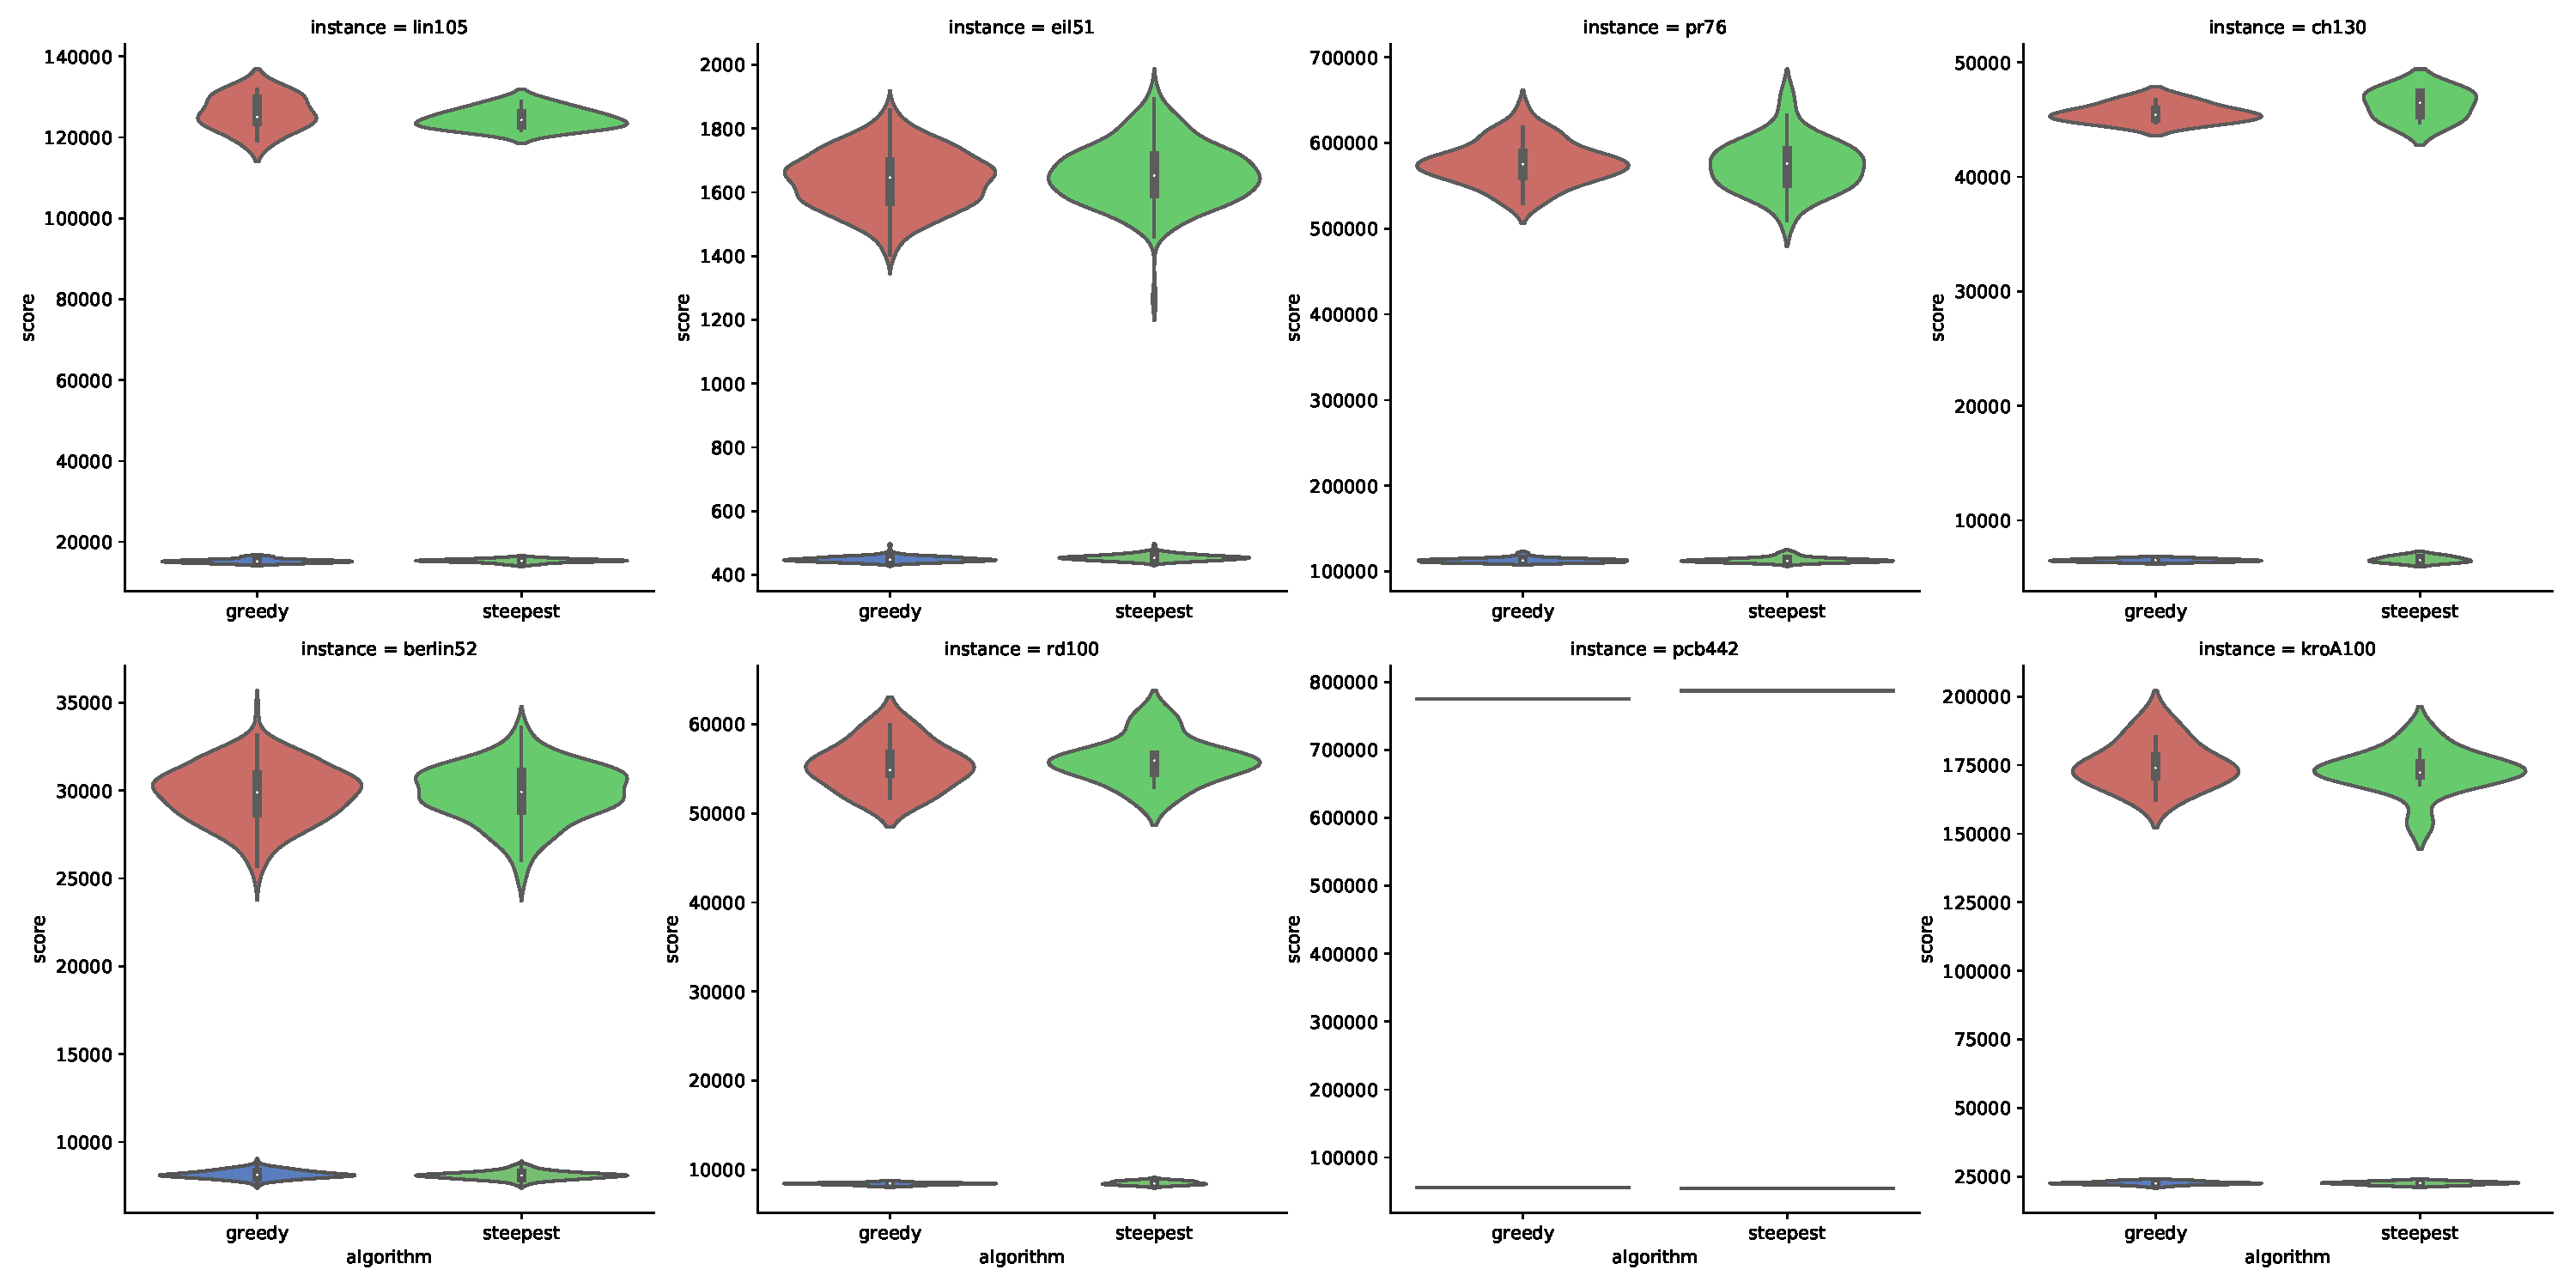
\includegraphics[width=1.0\textwidth]{graphs/init_vs_final_score_violin.pdf}
\end{center}
\caption{Porównanie jakości rozwiązań początkowych i~końcowych przez~algorytmy Greedy Search i~Steepest.}
\label{fig:diff}
\end{figure}

\subsubsection{Wielokrotne uruchamianie dla różnych rozwiązań początkowych}

Wykresy~\ref{fig:more_berlin} i~\ref{fig:more_eil} przedstawiają wartość najlepszego znalezionego rozwiązania po~i-tej iteracji. Jak~widać, poprawia się ona~co~pewien czas. Im~rozwiązanie jest lepsze, tym~ten~czas jest~dłuższy. Im~więcej razy algorytm będzie uruchamiany z~różnych rozwiązań początkowych, tym~istnieje większa szansa, że~osiągnie on~lepszy wynik, więc~warto powtarzać uruchomienia dla~różnych rozwiązań początkowych, aby~pełniej przeszukać przestrzeń wszystkich rozwiązań.

\begin{figure}[H]
\begin{center}
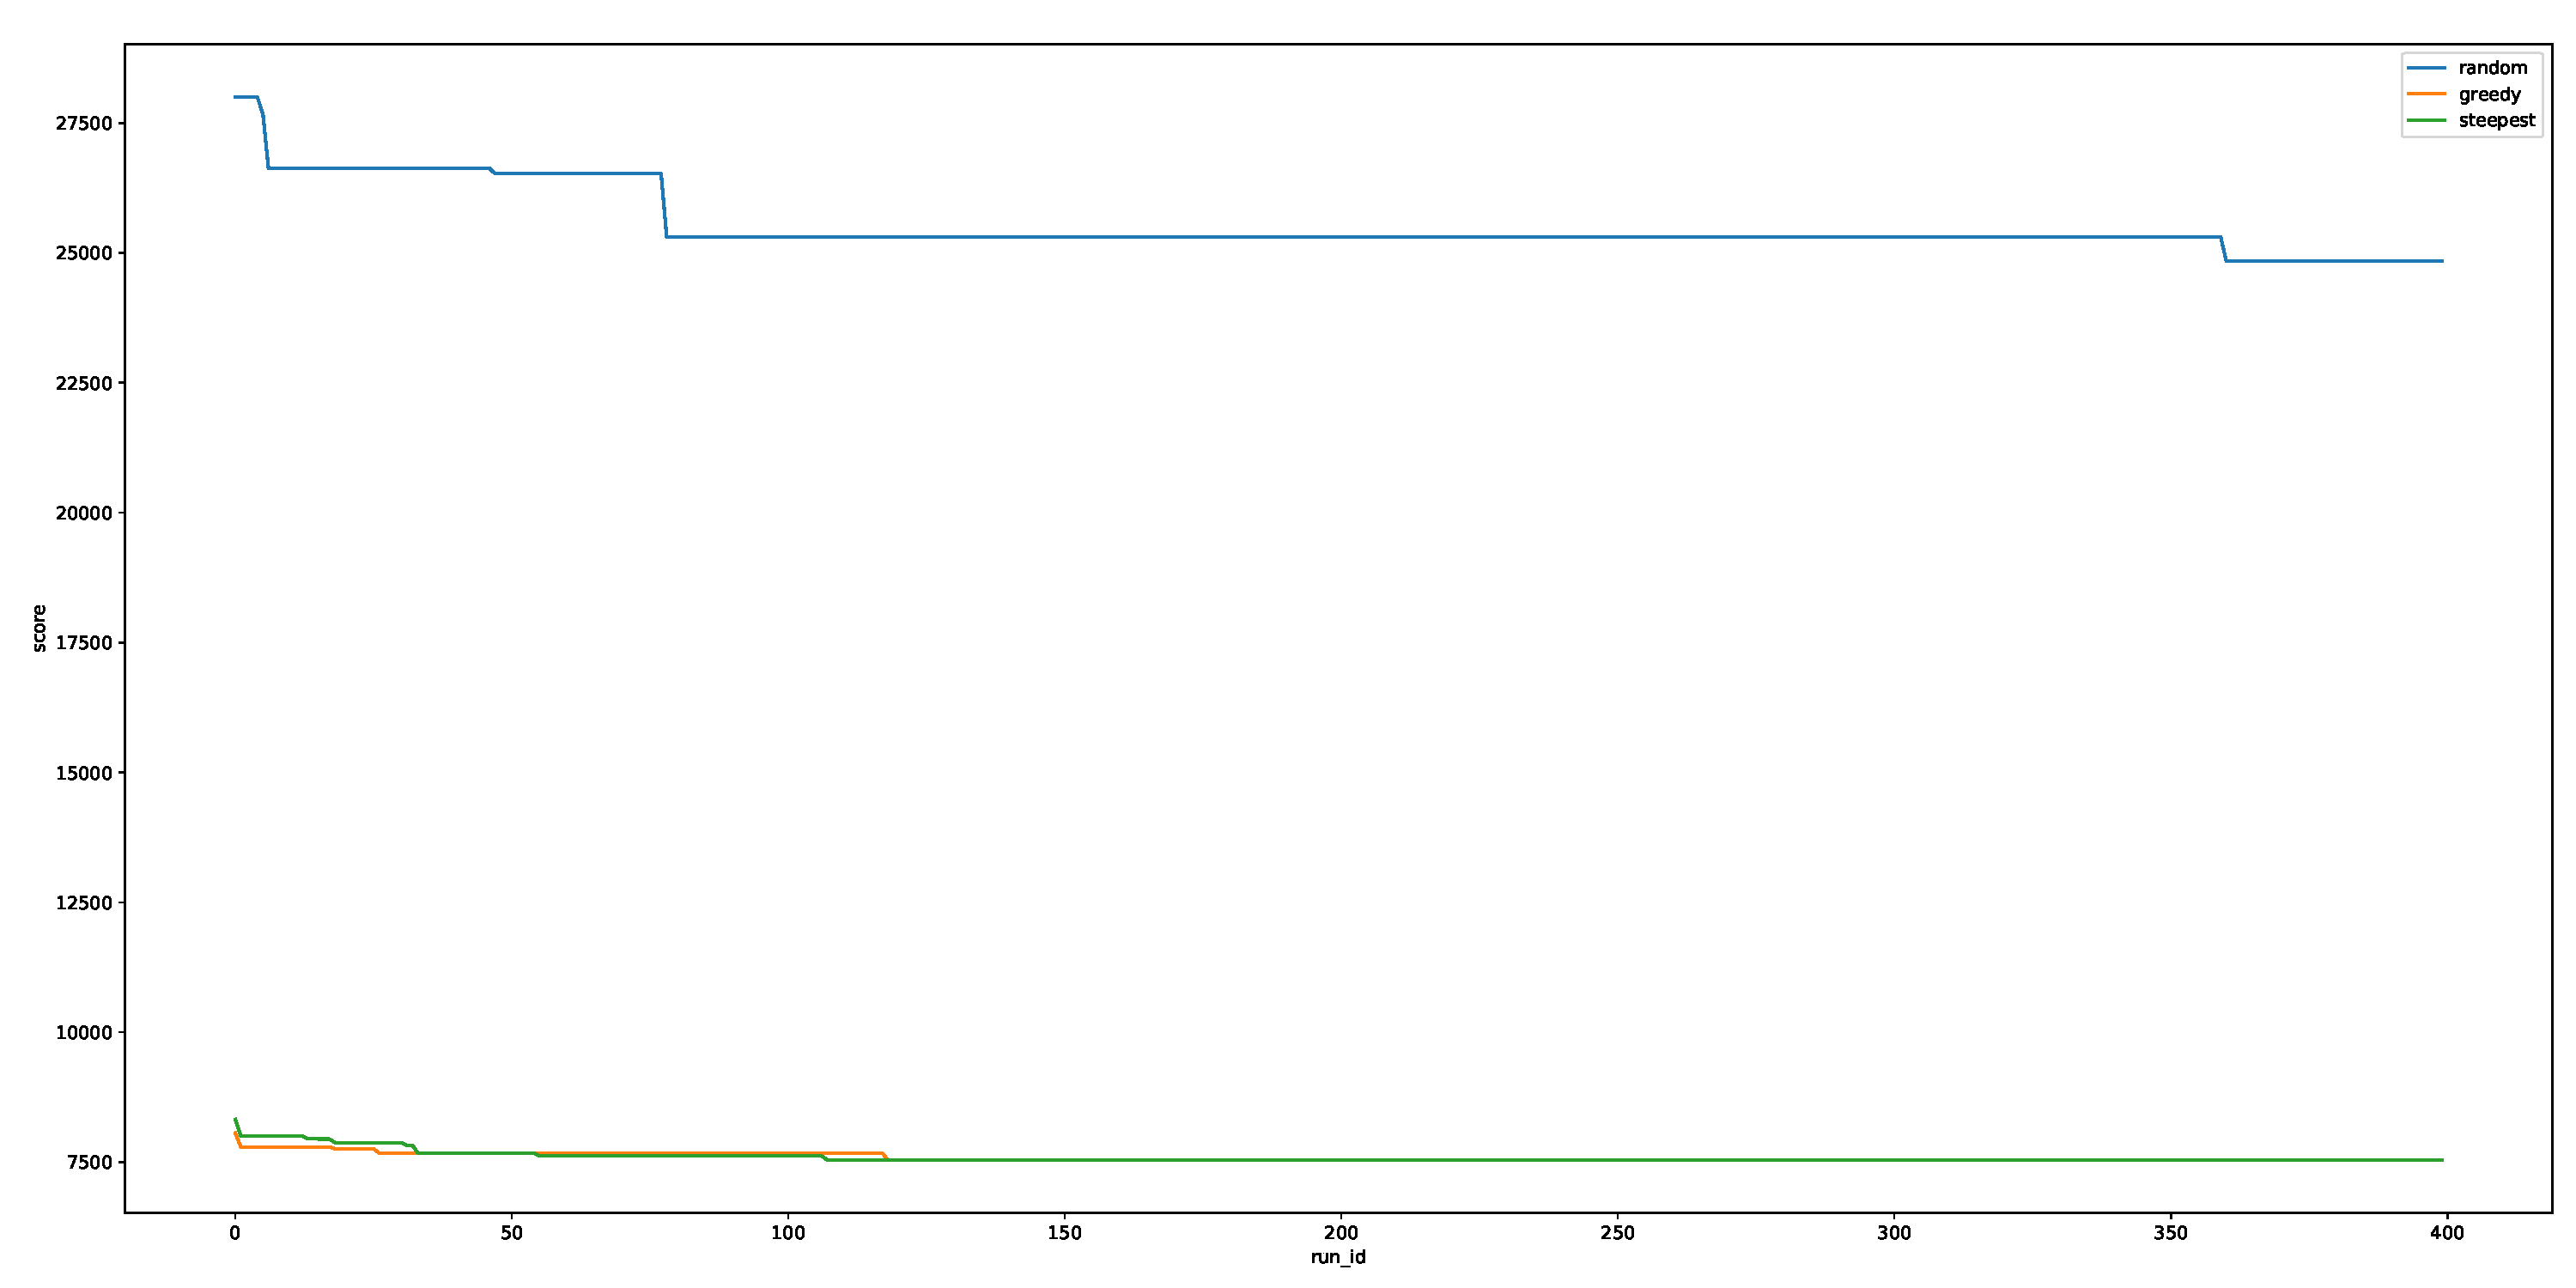
\includegraphics[width=1.0\textwidth]{graphs/multi_start_scoreberlin52.pdf}
\end{center}
\caption{Porównanie jakości rozwiązań algorytmów Gready Search i~Steepest w~zależności od~liczby uruchomień tych algorytmów dla~różnych rozwiązań początkowych dla~zbioru berlin52.}
\label{fig:more_berlin}
\end{figure}

\begin{figure}[H]
\begin{center}
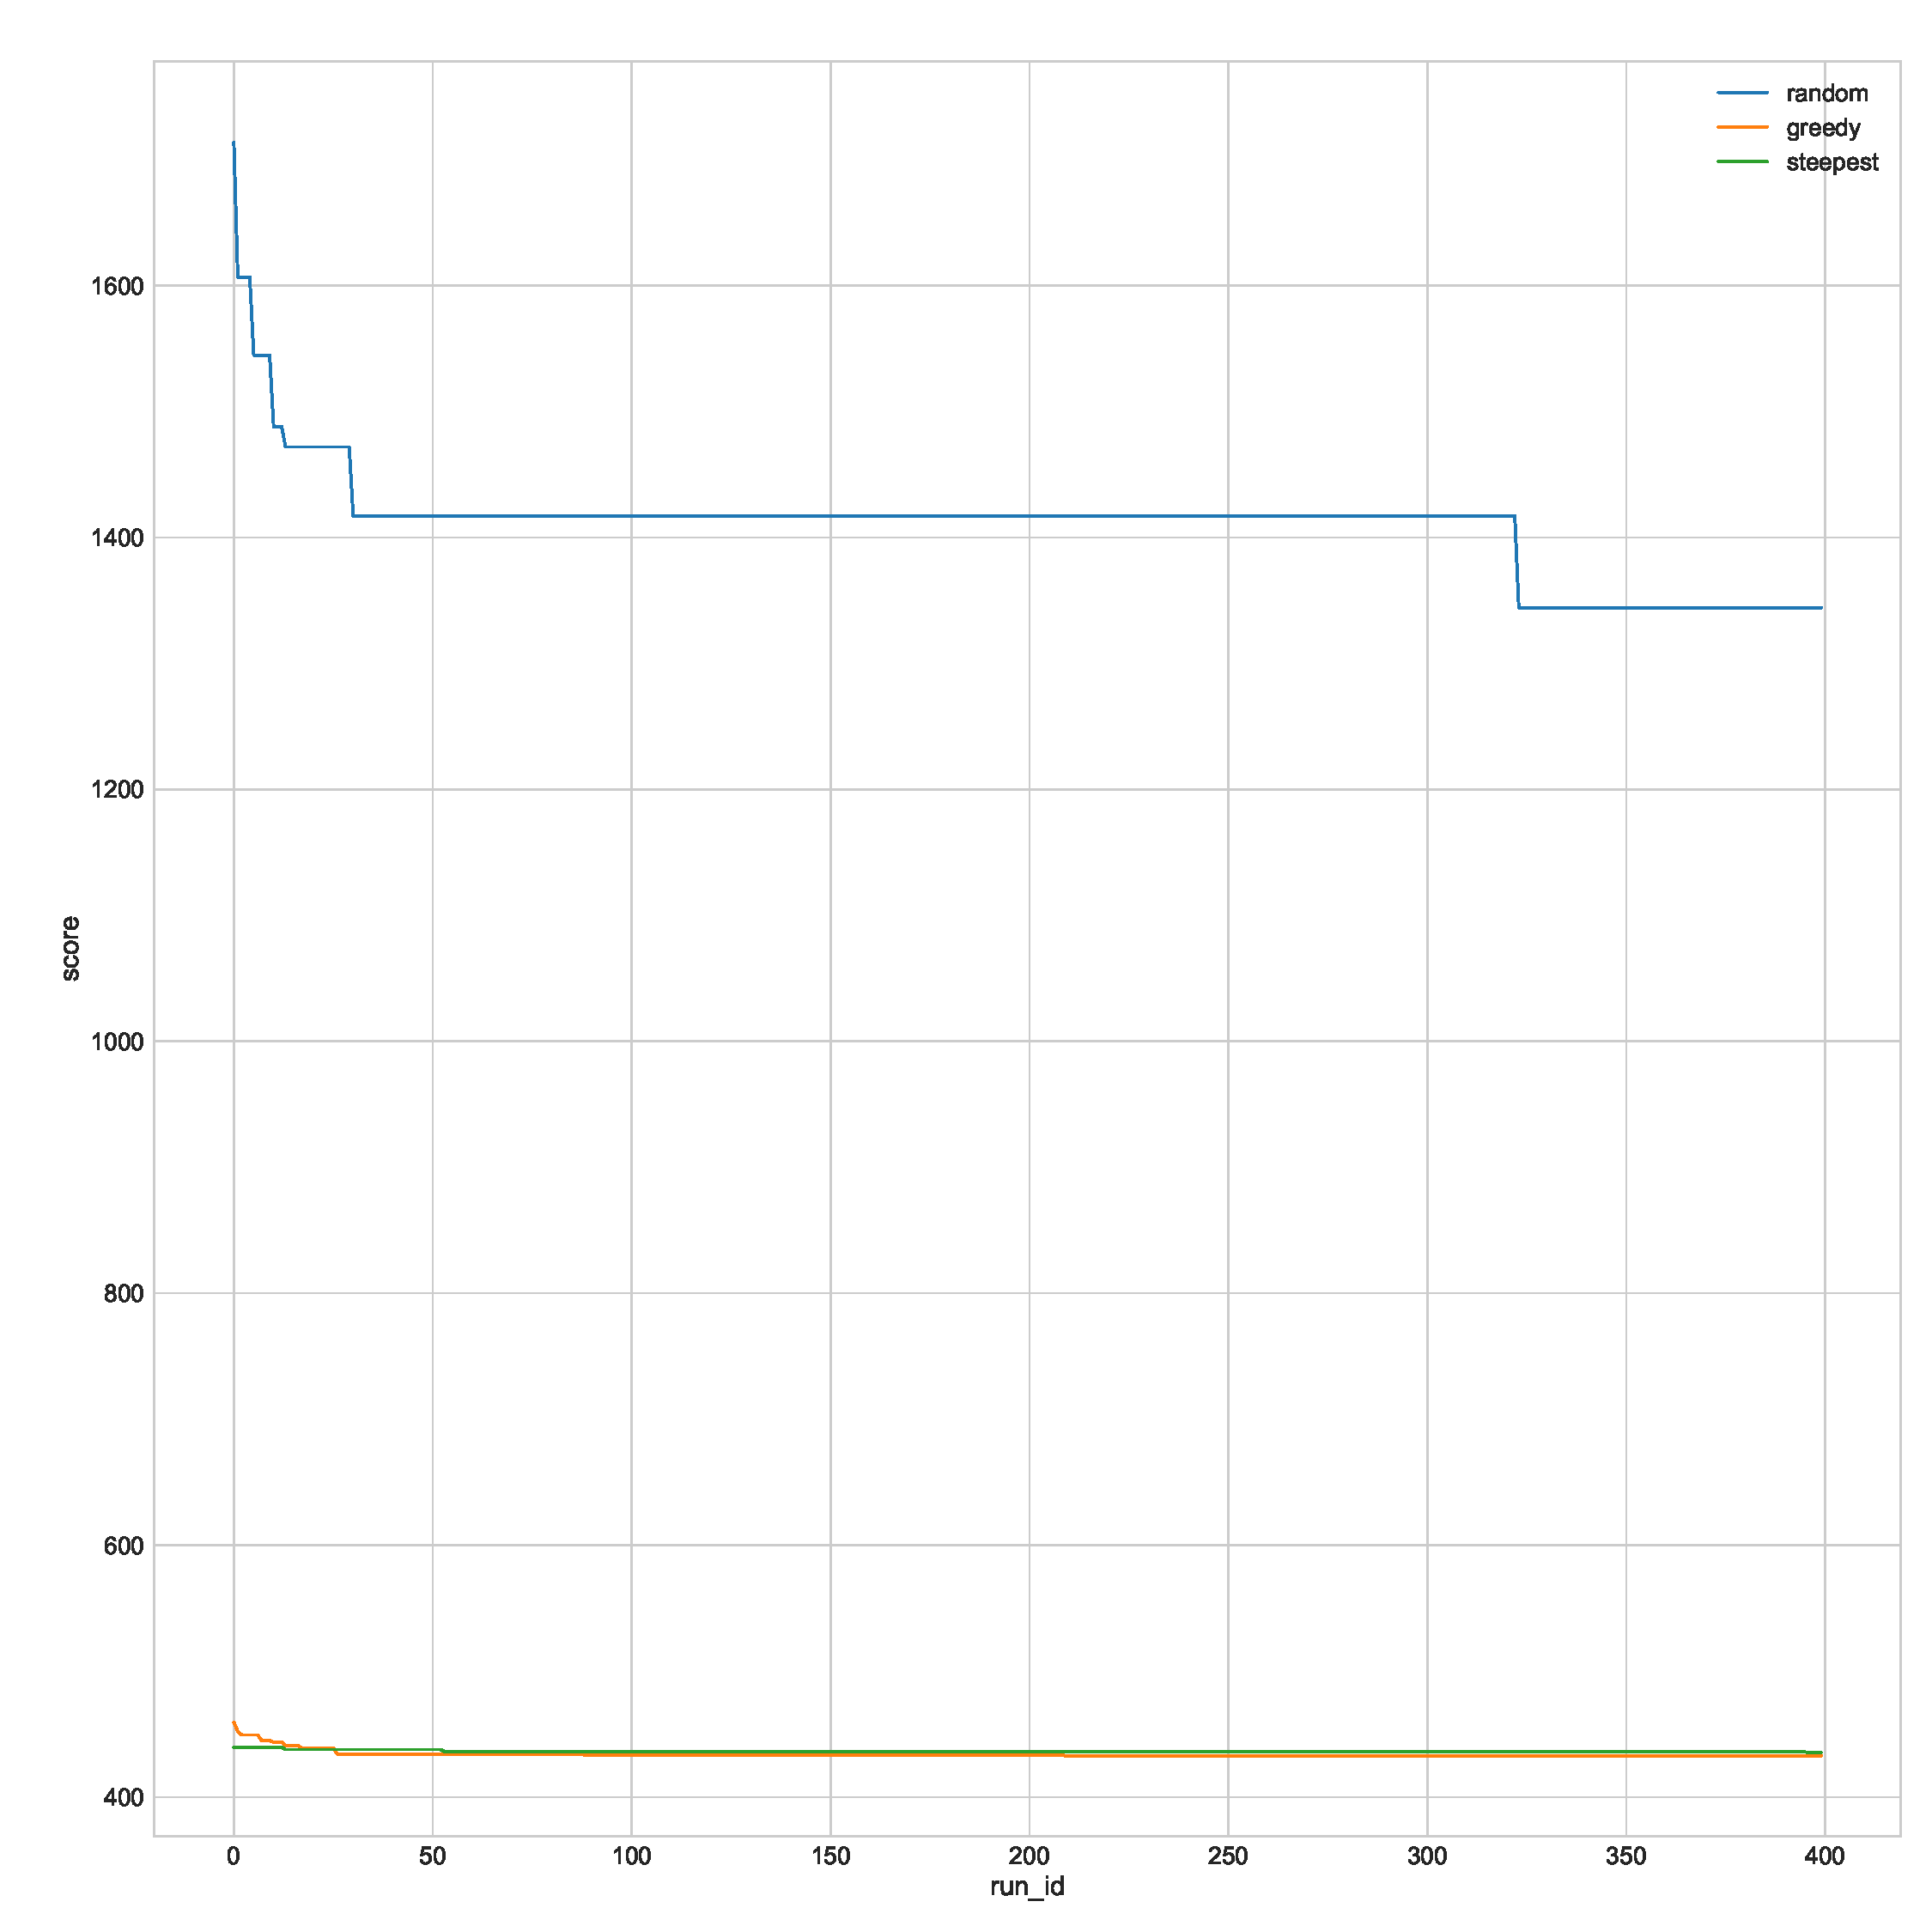
\includegraphics[width=1.0\textwidth]{graphs/multi_start_scoreeil51.pdf}
\end{center}
\caption{Porównanie jakości rozwiązań algorytmów Gready Search i~Steepest w~zależności od~liczby uruchomień tych algorytmów dla~różnych rozwiązań początkowych dla~zbioru eil51.}
\label{fig:more_eil}
\end{figure}

\subsection{Porównanie rozwiązań}

\subsubsection{Miara odległości rozwiązań od rozwiązania optymalnego}

Aby~porównywać między sobą rozwiązania, postanowiliśmy badać, jak~wiele mają takich samych krawędzi. Aby~to~zmierzyć, dla~każdej krawędzi w~jednym rozwiązaniu, sprawdzamy, czy~istnieje ona~w~drugim (skierowana w~dowolną stronę, ponieważ obie krawędzie są~symetryczne).

\subsubsection{Wyniki}

Na~rysunku~\ref{fig:sim} można zaobserwować podobieństwo rozwiązań znajdowanych przez algorytmy do~rozwiązania optymalnego. Istnieje wyraźna zależność polegająca na~tym, że~im~lepsze rozwiązanie, tym~jest~bardziej podobne do~optymalnego.

Bardzo mocno wyróżnia się chmura rozwiązań losowych --- jakość rozwiązań jest~bardzo różnorodna, ale~wszystkie są~bardzo mało podobne do~rozwiązania optymalnego (poniżej 10\%, a~im~więcej miast w~instancji, tym~mniej podobne).

\begin{figure}[H]
\begin{center}
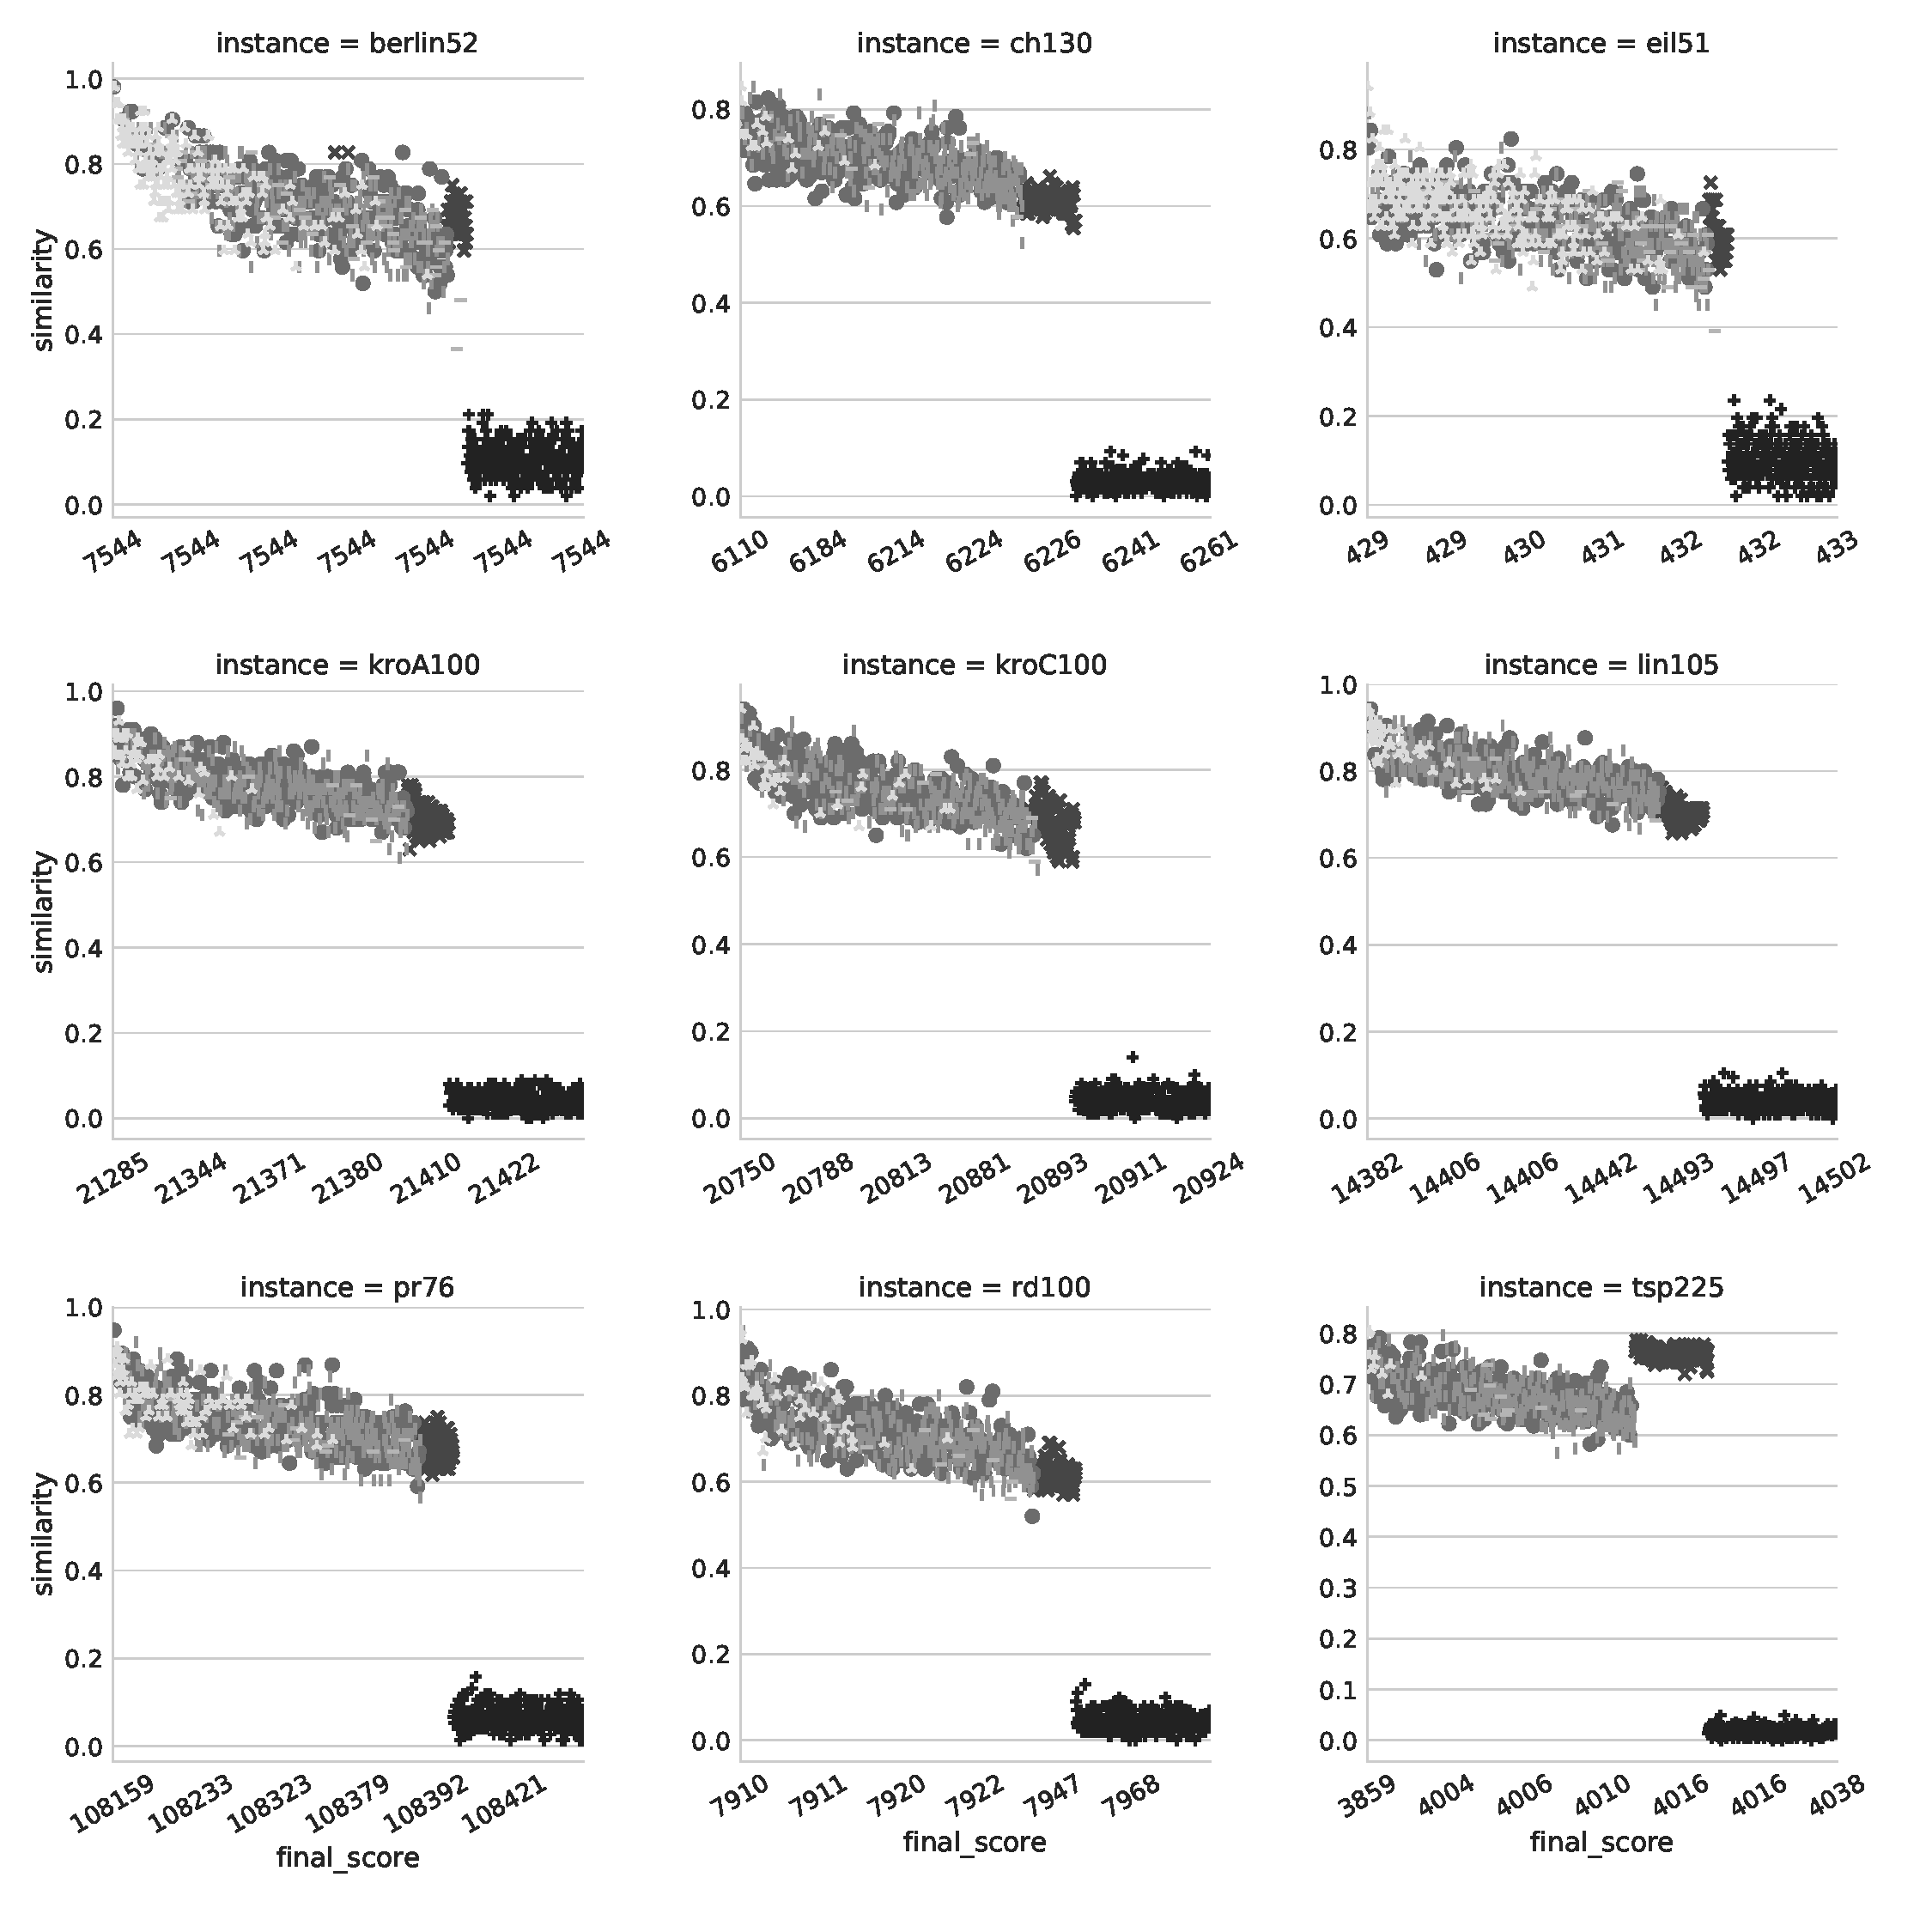
\includegraphics[width=1.0\textwidth]{graphs/similarity_comparision.pdf}
\end{center}
\caption{Porównanie odległości znajdowanych rozwiązań przez algorytmy od~rozwiązania optymalnego.}
\label{fig:sim}
\end{figure} %ML

\clearpage

\section{Podsumowanie}

%wnioski (od ogólnych do szczegółowych) z przeprowadzonych doświadczeń
%trudności na jakie napotkano
%uzasadnienie wprowadzanych ulepszeń, propozycje udoskonaleń i ich spodziewane efekty
\subsection{Wnioski}

W problemie symetrycznego komiwojażera, stosunkowo łatwo znaleźć dość dobre rozwiązanie za pomocą prostej heurystyki, którą też można jeszcze udoskonalić.

Algorytmy przeszukiwania lokalnego przeważnie znajdują jednak jeszcze lepsze rozwiązania, nieraz nawet optymalne (przy instancjach o liczności ok. 50 miast), pracując wielokrotnie dłużej, jednak wciąż nie dłużej niż minutę dla wybranych instancji. Algorytmy przeszukiwania lokalnego mimo, że zaczynają ze stosunkowo słabym rozwiązaniem losowym, wciąż poszukując lepszych w jego sąsiedztwie, potrafią osiągać bardzo dobre wyniki.

Porównując algorytmy Greedy i Steepest, można zauważyć, że ostatecznie oba zwracają podobnej jakości rozwiązania. Steepest wykonuje kilkakrotnie mniej kroków, jednak w każdym z nim musi przeszukać całe sąsiedztwo aktualnego rozwiązania, w konsekwencji czego, sumarycznie, przeszukuje większą przestrzeń rozwiązań i trwa dłużej od algorytmu Greedy. Zaobserwowaliśmy, że ta tendencja jest odwrotna dla dla największej, wybranej instancji.

\subsection{Trudności}

Jednym z głównych problemów, jakie wystąpiły podczas prezentacji wyników, było odpowiednie dobranie wykresów. Mimo, że 3 z 4 prezentowanych algorytmów dawało zbliżone wyniki, to random zawsze znacznie się od nich różnił, przez co trudno było tak wyskalować wykresy, aby wyraźnie było widać wszystkie zależności. 

Innym problemem jest odpowiednie dobranie parametrów, aby każdy algorytm został uruchomiony odpowiednią liczbę razy dla każdej instancji, ale jednocześnie, by generowanie obliczenia nie trwały zbyt długo.

\subsection{Propozycje udoskonaleń}

Warta zbadania na pewno jest sytuacja zaobserwowana dla największej instancji, w której Steepest okazuje się być lepszy od algorytmu Greedy pod względem czasu wykonania, przegląda też mniejszą liczbę rozwiązań. Warto sprawdzić, czy ta tendencja utrzymuje się dla przykładów z większą liczbą miast. %PG

%%%%%%%%%%%%%%%% literatura %%%%%%%%%%%%%%%%

\bibliography{sprawozd}
\bibliographystyle{plain}

\end{document}